\documentclass[12pt]{article}\usepackage[]{graphicx}\usepackage[]{color}
%% maxwidth is the original width if it is less than linewidth
%% otherwise use linewidth (to make sure the graphics do not exceed the margin)
\makeatletter
\def\maxwidth{ %
  \ifdim\Gin@nat@width>\linewidth
    \linewidth
  \else
    \Gin@nat@width
  \fi
}
\makeatother

\definecolor{fgcolor}{rgb}{0.345, 0.345, 0.345}
\newcommand{\hlnum}[1]{\textcolor[rgb]{0.686,0.059,0.569}{#1}}%
\newcommand{\hlstr}[1]{\textcolor[rgb]{0.192,0.494,0.8}{#1}}%
\newcommand{\hlcom}[1]{\textcolor[rgb]{0.678,0.584,0.686}{\textit{#1}}}%
\newcommand{\hlopt}[1]{\textcolor[rgb]{0,0,0}{#1}}%
\newcommand{\hlstd}[1]{\textcolor[rgb]{0.345,0.345,0.345}{#1}}%
\newcommand{\hlkwa}[1]{\textcolor[rgb]{0.161,0.373,0.58}{\textbf{#1}}}%
\newcommand{\hlkwb}[1]{\textcolor[rgb]{0.69,0.353,0.396}{#1}}%
\newcommand{\hlkwc}[1]{\textcolor[rgb]{0.333,0.667,0.333}{#1}}%
\newcommand{\hlkwd}[1]{\textcolor[rgb]{0.737,0.353,0.396}{\textbf{#1}}}%
\let\hlipl\hlkwb

\usepackage{framed}
\makeatletter
\newenvironment{kframe}{%
 \def\at@end@of@kframe{}%
 \ifinner\ifhmode%
  \def\at@end@of@kframe{\end{minipage}}%
  \begin{minipage}{\columnwidth}%
 \fi\fi%
 \def\FrameCommand##1{\hskip\@totalleftmargin \hskip-\fboxsep
 \colorbox{shadecolor}{##1}\hskip-\fboxsep
     % There is no \\@totalrightmargin, so:
     \hskip-\linewidth \hskip-\@totalleftmargin \hskip\columnwidth}%
 \MakeFramed {\advance\hsize-\width
   \@totalleftmargin\z@ \linewidth\hsize
   \@setminipage}}%
 {\par\unskip\endMakeFramed%
 \at@end@of@kframe}
\makeatother

\definecolor{shadecolor}{rgb}{.97, .97, .97}
\definecolor{messagecolor}{rgb}{0, 0, 0}
\definecolor{warningcolor}{rgb}{1, 0, 1}
\definecolor{errorcolor}{rgb}{1, 0, 0}
\newenvironment{knitrout}{}{} % an empty environment to be redefined in TeX

\usepackage{alltt}%[final]
\setcounter{secnumdepth}{3}
% if you need to pass options to natbib, use, e.g.:
% \PassOptionsToPackage{numbers, compress}{natbib}
% before loading nips_2016
%
% to avoid loading the natbib package, add option nonatbib:
% \usepackage[nonatbib]{nips_2016}

%\usepackage{nips_2016}

% to compile a camera-ready version, add the [final] option, e.g.:
%\usepackage[final]{nips_2016}
\usepackage{amsmath}
\usepackage[utf8]{inputenc} % allow utf-8 input
\usepackage[T1]{fontenc}    % use 8-bit T1 fonts
\usepackage{hyperref}       % hyperlinks
\usepackage{url}            % simple URL typesetting
\usepackage{booktabs}       % professional-quality tables
\usepackage{amsfonts}       % blackboard math symbols
\usepackage{nicefrac}       % compact symbols for 1/2, etc.
\usepackage{microtype}      % microtypography
\usepackage{float}
\usepackage{amssymb}
\usepackage{amsthm}
\usepackage{color,soul}
\usepackage{amsmath}
\usepackage{algorithm}
\usepackage[noend]{algpseudocode}
\usepackage[margin=1.5in]{geometry}
\usepackage[english]{babel}
\usepackage{graphicx}
\usepackage{longtable}
\usepackage{verbatim}
\usepackage{setspace}
\doublespacing

\newtheorem{theorem}{Theorem}[section]
\newtheorem{lemma}[theorem]{Lemma}
\newtheorem{proposition}[theorem]{Proposition}
\newtheorem{corollary}[theorem]{Corollary}
\theoremstyle{definition}
\newtheorem{definition}{Definition}[section]

% Code defs from jss
\newcommand\code{\@codex}
\def\@codex#1{{\normalfont\ttfamily\hyphenchar\font=-1 #1}}
%%\let\code=\texttt
\let\proglang=\textsf
\newcommand{\pkg}[1]{{\fontseries{b}\selectfont #1}}


%\theoremstyle{definition}
%\newtheorem{definition}{Definition}[section]


\makeatletter
\def\BState{\State\hskip-\ALG@thistlm}
\makeatother

\title{Time Series Methods in the R package \pkg{mlr}}

% The \author macro works with any number of authors. There are two
% commands used to separate the names and addresses of multiple
% authors: \And and \AND.
%
% Using \And between authors leaves it to LaTeX to determine where to
% break the lines. Using \AND forces a line break at that point. So,
% if LaTeX puts 3 of 4 authors names on the first line, and the last
% on the second line, try using \AND instead of \And before the third
% author name.

\author{
  Steve Bronder \\
  %Quantitative Methods of the Social Sciences\\
  %Columbia University\\
  %New York City, NY 10027 \\
  \texttt{sab2287@columbia.edu} \\
  %% examples of more authors test etst
   %Department of Computer Science \\
   %Columbia University\\
   %New York City, NY 10027 \\
  %% \AND
  %% Coauthor \\
  %% Affiliation \\
  %% Address \\
  %% \texttt{email} \\
  %% \And
  %% Coauthor \\
  %% Affiliation \\
  %% Address \\
  %% \texttt{email} \\
  %% \And
  %% Coauthor \\
  %% Affiliation \\
  %% Address \\
  %% \texttt{email} \\
}
\IfFileExists{upquote.sty}{\usepackage{upquote}}{}
\begin{document}
% \nipsfinalcopy is no longer used

\maketitle

\begin{abstract}
The \pkg{mlr} package is a unified interface for machine learning tasks such as classification, regression, cluster analysis, and survival analysis. \pkg{mlr} handles the data pipeline of preprocessing, resampling, model selection, model tuning, ensembling, and prediction. This paper details new methods for developing time series  models in \pkg{mlr}. It includes standard and novel tools such as autoregressive and LambertW transform data generating processes, fixed and growing window cross validation, and forecasting models in the context of univariate and multivariate time series. Examples from forecasting competitions will be given in order to demonstrate the benefits of a unified framework for machine learning and time series.
  \end{abstract}


\section{Introduction}
There has been a rapid developement in time series methods over the last 25 years ~\cite{Hyndman25} whereby time series models have not only become more common, but more complex. The \proglang{R} language ~\cite{Rbase} has several task views with compiling the packages available for forecasting, time series methods, and applied finance. However, the open source nature of R has left users without a standard framework. Many packages have their own sub-culture of style, syntax, and output. The \pkg{mlr} ~\cite{mlr} package, short for Machine Learning in R, works to give a strong syntatic framework for the modeling pipeline. By automating many of the standard tools in machine learning such as preprocessing and cross validation, \pkg{mlr} reduces error from the user during the modeling process. 

While there are some time series methods available in \pkg{caret} ~\cite{caret}, development of forecasting models in \pkg{caret} is difficult due to computational constraints and design choices within the package. The highly modular structure of \pkg{mlr} makes it the best choice for implementing time series methods and models. This paper will show how using \pkg{mlr}'s strong syntatic structure allows for time series packages such as \pkg{forecast} ~\cite{HyndForecast}, \pkg{rugarch} ~\cite{rugarch}, and \pkg{BigVAR} ~\cite{BigVAR} to use machine learning methedologies such as automated parameter tuning, data preprocessing, model blending, cross validation, performance evaluation, and parallel processing techniques for decreasing model build time.

\section{Forecasting Example with the M4 Competition}
\label{sec:m4data}

Professional forecasters attempt to predict the future of a series based on its past values. Forecasting can be used in a wide range of tasks including forecasting stock prices, ~\cite{GRANGER19923}, weather patterns ~\cite{MurphymeteoForecast}, international conficts ~\cite{Chadefaux01012014}, and earthquakes ~\cite{earthquakeYegu}. In order to evaluate \pkg{mlr}'s forecasting framework we need a large set of possible time series to make sure our methods generalize well.

The Makridakis competition ~\cite{Makridakis2000451} is a set of forecasting challenges organized by the International Institute of Forecasters and led by Spyros Makridakis to evaluate and compare the accuracy of forecasting methods. The most recent of the competitions, the M4 competition, contains 10,000 time series on a yearly, quarterly, monthly, and daily frequency in areas such as finance, macroeconomics, climate, microeconomics, and industry. To show examples of how \pkg{mlr}'s forecasting features works we will look at a particular climate series. The data is daily with the training subset starting on September 6th, 2007 and ending on September 5th, 2009 while the testing subset is from September 6th, 2009 to October 10th, 2009 for a total of 640 training periods and 35 test periods to forecast.

\singlespacing
\begin{knitrout}
\definecolor{shadecolor}{rgb}{0.969, 0.969, 0.969}\color{fgcolor}\begin{kframe}
\begin{alltt}
\hlkwd{library}\hlstd{(M4comp)}
\hlkwd{library}\hlstd{(xts)}
\hlkwd{library}\hlstd{(lubridate)}
\hlstd{m4.climate} \hlkwb{<-} \hlstd{M4[[}\hlnum{8836}\hlstd{]]}
\hlstd{m4.train} \hlkwb{<-} \hlkwd{xts}\hlstd{(m4.climate}\hlopt{$}\hlstd{past,} \hlkwd{as.POSIXct}\hlstd{(}\hlstr{"2007-12-05"}\hlstd{)} \hlopt{+} \hlkwd{days}\hlstd{(}\hlnum{0}\hlopt{:}\hlkwd{I}\hlstd{(}\hlkwd{length}\hlstd{(m4.climate}\hlopt{$}\hlstd{past)}\hlopt{-}\hlnum{1}\hlstd{)))}
\hlstd{m4.test} \hlkwb{<-} \hlkwd{xts}\hlstd{(m4.climate}\hlopt{$}\hlstd{future,} \hlkwd{as.POSIXct}\hlstd{(}\hlstr{"2009-09-06"}\hlstd{)} \hlopt{+} \hlkwd{days}\hlstd{(}\hlnum{0}\hlopt{:}\hlkwd{I}\hlstd{(}\hlkwd{length}\hlstd{(m4.climate}\hlopt{$}\hlstd{future)}\hlopt{-}\hlnum{1}\hlstd{)))}
\hlkwd{colnames}\hlstd{(m4.train)} \hlkwb{<-} \hlstr{"target_var"}
\hlkwd{colnames}\hlstd{(m4.test)} \hlkwb{<-} \hlstr{"target_var"}
\end{alltt}
\end{kframe}
\end{knitrout}

\begin{knitrout}
\definecolor{shadecolor}{rgb}{0.969, 0.969, 0.969}\color{fgcolor}

{\centering 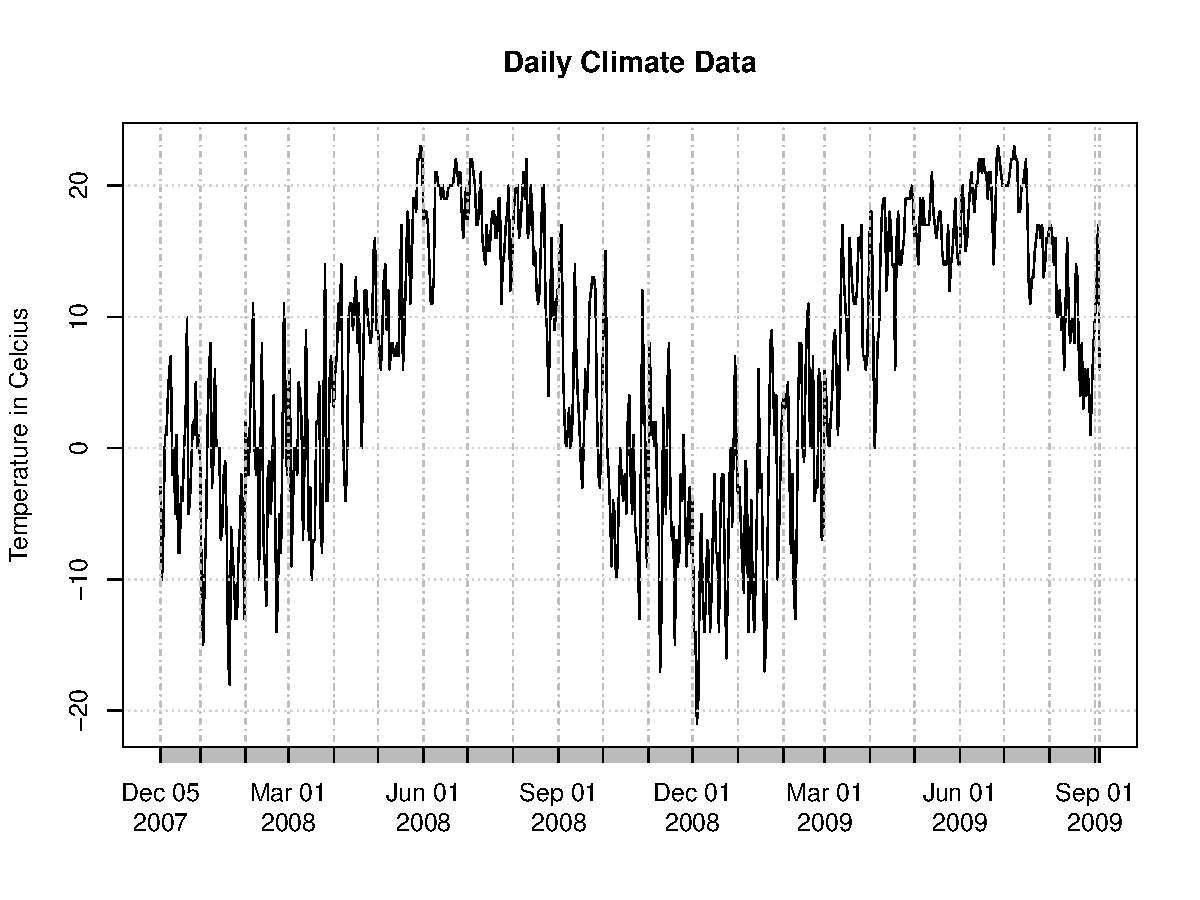
\includegraphics[width=\maxwidth]{figure/plot_dat_weather-1} 

}



\end{knitrout}
\doublespacing
This series was chosen for its obvious seasonality and time features. Some series in M4 only contain 12 observations, which is not enough data to accurately train a model. The example data set should be large enough that the tuning method can take multiple windows of the data. We can see figure one is what most people imagine when they think of a time series. There is a clear seasonal time trend with individual points moving about the seasonal periods. The data can be found in the package \pkg{M4comp} ~\cite{m4comp} under sets \code{M4[28]} and \code{M4[29]}. 

For multivariate forecasting, we will use the EUStockMarkets data set from the \pkg{datasets} ~\cite{datasets}. It contains a set of DAX, SMI, CAC, and FTSE European stock indices from July 1st, 1991 to August 24th, 1998 totaling 1828 training observations and 32 test observations.

\begin{knitrout}
\definecolor{shadecolor}{rgb}{0.969, 0.969, 0.969}\color{fgcolor}\begin{kframe}
\begin{alltt}
\hlkwd{data}\hlstd{(}\hlstr{"EuStockMarkets"}\hlstd{)}
\hlstd{EuStockMarkets.time} \hlkwb{=} \hlstd{lubridate}\hlopt{::}\hlkwd{date_decimal}\hlstd{(}\hlkwd{as.numeric}\hlstd{(}\hlkwd{time}\hlstd{(EuStockMarkets)))}
\hlstd{EuStockMarkets}  \hlkwb{=} \hlstd{xts}\hlopt{::}\hlkwd{xts}\hlstd{(}\hlkwd{as.data.frame}\hlstd{(EuStockMarkets),} \hlkwc{order.by} \hlstd{= EuStockMarkets.time)}
\hlstd{eu.train} \hlkwb{=} \hlstd{EuStockMarkets[}\hlnum{1}\hlopt{:}\hlnum{1828}\hlstd{,]}
\hlstd{eu.test} \hlkwb{=} \hlstd{EuStockMarkets[}\hlnum{1829}\hlopt{:}\hlnum{1860}\hlstd{,]}
\end{alltt}
\end{kframe}
\end{knitrout}

\begin{knitrout}
\definecolor{shadecolor}{rgb}{0.969, 0.969, 0.969}\color{fgcolor}

{\centering 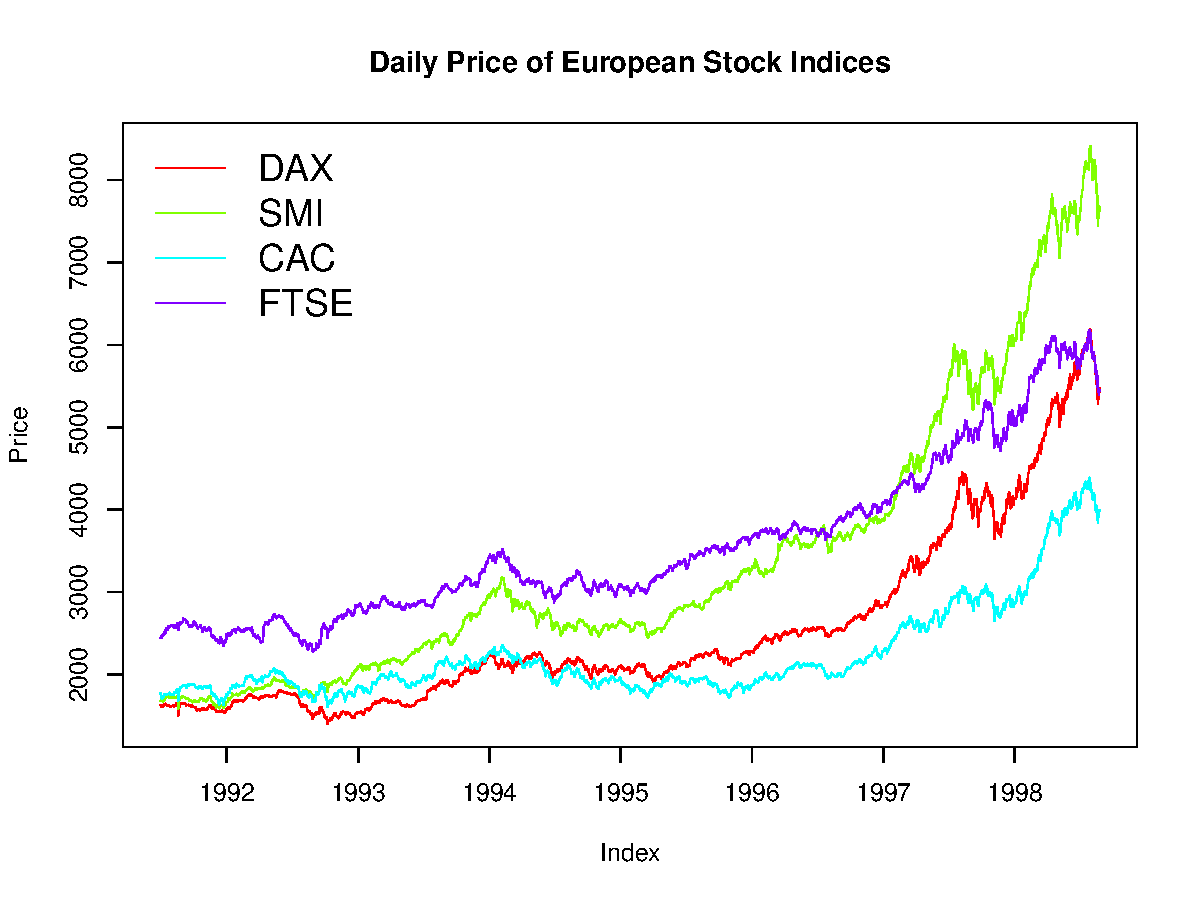
\includegraphics[width=\maxwidth]{figure/plot_dat_stocks-1} 

}



\end{knitrout}

Note that each stock index tends to follow a similar, but diverging, trend. This will be important to note when we perform windowing cross validation as it will let us see how well the models adapt to what appears to be nonstationary data.

\section{Univariate and Multivariate Forecasting Tasks}
\label{sec:task}

\section{Univariate Tasks}

\pkg{mlr} uses the S3 object system to clearly define a predictive modeling task. Tasks contain the data and other relevant information such as the task id and which variable you are targeting for supervised learning problems. Forecasting tasks are handled in \pkg{mlr} by the function \code{makeForecastRegrTask()}. The forecasting task inherets most of it's arguments from \code{makeRegrTask}, but has two noticable differences in arguments.

\begin{itemize}
\item[data:] Instead of a data frame, an xts object from \pkg{xts} ~\cite{xts} containing the time series.
\item[frequency:] An integer with the periodicity of the time series. For example, daily data with a weekly periodicity has a frequency of 7, daily data with a yearly periodicity has a frequency of 365, and weekly data with a yearly frequency has a periodicity of 52.
\end{itemize}

\singlespacing
\begin{knitrout}
\definecolor{shadecolor}{rgb}{0.969, 0.969, 0.969}\color{fgcolor}\begin{kframe}
\begin{alltt}
\hlkwd{library}\hlstd{(mlr)}

\hlstd{climate.task} \hlkwb{=} \hlkwd{makeForecastRegrTask}\hlstd{(}\hlkwc{id} \hlstd{=} \hlstr{"M4 Climate Data"}\hlstd{,}
                                 \hlkwc{data} \hlstd{= m4.train,}
                                 \hlkwc{target} \hlstd{=} \hlstr{"target_var"}\hlstd{,}
                                 \hlkwc{frequency} \hlstd{=} \hlnum{183L}\hlstd{)}
\hlstd{climate.task}
\end{alltt}
\begin{verbatim}
## Task: M4 Climate Data
## Type: fcregr
## Target: target_var
## Observations: 640
## Dates:
##  Start: 2007-12-05 
##  End:   2009-09-04
## Frequency: 183
## Features:
## numerics  factors  ordered 
##        0        0        0 
## Missings: FALSE
## Has weights: FALSE
## Has blocking: FALSE
\end{verbatim}
\end{kframe}
\end{knitrout}
\doublespacing
Like a regression task, this records the type of the learning problem and basic information about the data set such as the start and end dates, frequency, and whether we have missing values. Note that there are zero features in our task because we only have a target variable, which the model itself will use to build features.

\subsection{Multivariate Tasks}

One common problem with forecasting is that it is difficult to use additional explanatory variables or forecast multiple targets that are dependent on one another. If we are at time $t$ and want to forecast 10 periods in the future, we need to know the values of the explanatory variables at time $t+10$, which is often not possible. A new set of models ~\cite{BigVAR} which treats explanatory variables endogenously instead of exogenously allows us to forecast not only our target, but addititional explanatory variables. This is done by treating all the variables as targets, making them endogeneous to the model. To use these models, we create a multivariate forecasting task. The function \code{makeMultiForecastRegrTask()} has the same arguments as \code{makeForecastRegrTask()} with one exception. The \code{target} argument can contain either a single target variable, multiple target variables, or \code{All} which treats all variables endogeneously.
\singlespacing
\begin{knitrout}
\definecolor{shadecolor}{rgb}{0.969, 0.969, 0.969}\color{fgcolor}\begin{kframe}
\begin{alltt}
\hlstd{mfcregr.univar.task} \hlkwb{=} \hlkwd{makeMultiForecastRegrTask}\hlstd{(}\hlkwc{id} \hlstd{=} \hlstr{"bigvar"}\hlstd{,}
                                                \hlkwc{data} \hlstd{= EuStockMarkets,}
                                                \hlkwc{target} \hlstd{=} \hlstr{"FTSE"}\hlstd{,}
                                                \hlkwc{frequency} \hlstd{=} \hlnum{365L}\hlstd{)}
\hlstd{mfcregr.univar.task}
\end{alltt}
\begin{verbatim}
## Task: bigvar
## Type: mfcregr
## Target: FTSE
## Observations: 1860
## Dates:
##  Start: 1991-07-01 02:18:27 
##  End:   1998-08-24 20:18:27
## Frequency: 365
## Features:
## numerics  factors  ordered 
##        3        0        0 
## Missings: FALSE
## Has weights: FALSE
## Has blocking: FALSE
\end{verbatim}
\end{kframe}
\end{knitrout}
\doublespacing

Like \code{makeForecastRegrTask()}, \code{mfcregr.univar.task} has the standard output, but notice now that there are three features. Alternatively, \code{mfcregr.all.task} contains multiple target values with no features. The difference between each of these multivariate tasks is that \code{mfcregr.univar.task} will act similar to \code{makeForecastRegrTask()}, giving the output, predictions, and even using the measures for univariate forecasting tasks. Both of these tasks will still forecast all of the underlying series, which allows us take exogeneous models and treat them endogeneously for n-step forecasts that use additional explanatory variables.

\singlespacing
\begin{knitrout}
\definecolor{shadecolor}{rgb}{0.969, 0.969, 0.969}\color{fgcolor}\begin{kframe}
\begin{alltt}
\hlstd{mfcregr.all.task} \hlkwb{=} \hlkwd{makeMultiForecastRegrTask}\hlstd{(}\hlkwc{id} \hlstd{=} \hlstr{"bigvar"}\hlstd{,}
                                             \hlkwc{data} \hlstd{= eu.train,}
                                             \hlkwc{target} \hlstd{=} \hlstr{"all"}\hlstd{,}
                                             \hlkwc{frequency} \hlstd{=} \hlnum{365L}\hlstd{)}
\hlstd{mfcregr.all.task}
\end{alltt}
\begin{verbatim}
## Task: bigvar
## Type: mfcregr
## Target: DAX SMI CAC FTSE
## Observations: 1828
## Dates:
##  Start: 1991-07-01 02:18:27 
##  End:   1998-07-10 22:09:13
## Frequency: 365
## Features:
## numerics  factors  ordered 
##        0        0        0 
## Missings: FALSE
## Has weights: FALSE
## Has blocking: FALSE
\end{verbatim}
\end{kframe}
\end{knitrout}
\doublespacing

\section{Building and Tuning a forecast learner}

\subsection{Univariate Forecasting}

The \code{makeLearner()} function provides a structured model building framework to the several forecasting models currently implimented in \pkg{mlr}. As an example, we will build the Trigonometric exponential smoothing state space model with Box-Cox transformation, ARMA errors, Trend and Seasonal Components (TBATS)~\cite{tbats}.
\begin{comment}
To create the original BATS model we let $y_t^{\omega}$ be a box cox transformed observation with parameter $\omega$. Then let $m_T$ be the seasonal periods, $l_t$ be the local level in the period, $b$ the long term trend with $b_t$ being the short term trend, $s_t^i$ being the $i$th seasonal component, $d_t$ being an ARIMA($p,q$) model with gaussian white noise process $\epsilon_t$. Smoothing parameters are given by $\alpha$, $\beta$, and $\gamma$ and $\phi$ is the damping constant of the trend.

\begin{align}
y_t^{\omega} &= \begin{cases} 
    \frac{y_t^{\omega} - 1}{\omega}, \omega \ne 0\\
    log(y_t), \omega = 0
    \end{cases}\\
y_t^{\omega} &= l_{t-1} + \phi b_{t-1} + \sum_{i=1}^T s_{t-m_i}^i + d_t\\
l_t &= l_{t-1} + \phi b_{t-1} + \alpha d_t \\
b_t &= (1-\phi)b + \phi b_{t-1} + \beta d_t \\
s_t^i &= s_{t-m_i}^i + \gamma_i d_t \\
d_t &= \sum_{i=1}^p \psi_i d_{t-i} + \sum_{i=1}^q \theta_i \epsilon_{t-i} + \epsilon
\end{align}

The trigonometric part of the model comes from the representation of the seasonal components based on fourier series ~\cite{fourierTrans}. Let the stochastic level of the $i$th seasonal component be $s_{j,t}^{(i)}$ and the stochastic growth in the level of the $i$th seasonal component that is needed to describe the change in the seasonal component over time by $s_{j,t}^{*(i)}$. 

\begin{align}
s_t^{(i)} &= \sum_{j=1}^{k_i} s_{j,t}^{(i)}\\
s_{j,t}^{(i)} &= s_{j,t-1}^{(i)} \cos\lambda_j^{(i)} + s_{j,t-1}^{(i)}\sin\lambda_j^{(i)} + \gamma_1^{(i)}d_t\\
s_{j,t}^{*(i)} &= -s_{j,t-1} \sin\lambda_j^{(i)} + s_{j,t-1}^{*(i)}\cos\lambda_j^{(i)} + \gamma_2^{(i)}d_t
\end{align}

The smoothing parameters are defined by $\gamma_1^{(i)}$ and $\gamma_2^{(i)}$ with $\lambda_j^{(i)} = 2\pi j/m_i$ being a trigonometric smoothing parameter associated with the seasonal periods. The parameter $k_i$ is number of harmonics necessary in the $i$th seasonal component. It's possible to show a simpler deterministic representation of the seasonal components by setting the smoothing parameters to zero. The TBATS model is created by replacing the seasonal component $s_t^{(i)}$ in equation 5 with the trigonometric seasonal equations as well as replacing the measure equation in 2 with 

\begin{equation}
y_t^{\omega} = l_{t-1} + \phi b_{t-1} + \sum_{i=1}^T s_{t-1}^{(i)} + d_t
\end{equation}

\end{comment}

TBATS is one of the most well known forecasting models and is available in mlr along with models such as BATS, ARIMA, ETS, several GARCH variants, and autoregressive neural networks. In addition, preprocessing features have been added to allow arbitrary supervised machine learning models to be used in the context of forecasting. To impliment the TBATS model we use  \code{makeLearner()}, supplying the class of learner, order, the number of steps to forecast, and any additional arguments to be passed to \code{tbats} for \pkg{forecast}. 

\singlespacing
\begin{knitrout}
\definecolor{shadecolor}{rgb}{0.969, 0.969, 0.969}\color{fgcolor}\begin{kframe}
\begin{alltt}
\hlstd{tbats.mod} \hlkwb{=}\hlkwd{makeLearner}\hlstd{(}\hlstr{"fcregr.tbats"}\hlstd{,} \hlkwc{use.box.cox} \hlstd{=} \hlnum{TRUE}\hlstd{,}
                      \hlkwc{use.trend} \hlstd{=} \hlnum{TRUE}\hlstd{,}
                      \hlkwc{seasonal.periods} \hlstd{=} \hlnum{TRUE}\hlstd{,} \hlkwc{max.p} \hlstd{=} \hlnum{60}\hlstd{,} \hlkwc{max.q} \hlstd{=} \hlnum{60}\hlstd{,}
                      \hlkwc{stationary} \hlstd{=} \hlnum{FALSE}\hlstd{,} \hlkwc{use.arma.errors} \hlstd{=} \hlnum{TRUE}\hlstd{,}
                      \hlkwc{h} \hlstd{=} \hlnum{35}\hlstd{,} \hlkwc{predict.type} \hlstd{=} \hlstr{"response"}\hlstd{)}
\end{alltt}
\end{kframe}
\end{knitrout}
\doublespacing

We can also supply a predict type for forecasting models to either receive point estimates (\code{response}) or point estimates with quantiles of confidence intervals (\code{quantile}). To train the model we simply call train, supplying the forecasting model and task. After training the model it's simple to get our forecasts by calling \code{predict()} with the test data, returning an object containing meta information for the forecasts along with the prediction and test data in columns \code{truth} and \code{response}, respectively.

\singlespacing
\begin{knitrout}
\definecolor{shadecolor}{rgb}{0.969, 0.969, 0.969}\color{fgcolor}\begin{kframe}
\begin{alltt}
\hlstd{train.tbats}\hlkwb{=} \hlkwd{train}\hlstd{(}\hlkwc{learner} \hlstd{= tbats.mod,} \hlkwc{task} \hlstd{= climate.task )}
\hlstd{predict.tbats} \hlkwb{=} \hlkwd{predict}\hlstd{(train.tbats,} \hlkwc{newdata} \hlstd{= m4.test)}
\end{alltt}
\end{kframe}
\end{knitrout}
\doublespacing

To measure the performane of TBATS we call \code{performance()} with the Mean Absolute Scaled Error (MASE) ~\cite{Hyndman2006} measure.

\singlespacing
\begin{knitrout}
\definecolor{shadecolor}{rgb}{0.969, 0.969, 0.969}\color{fgcolor}\begin{kframe}
\begin{alltt}
\hlkwd{performance}\hlstd{(predict.tbats, mase,} \hlkwc{task} \hlstd{= climate.task)}
\end{alltt}
\begin{verbatim}
##      mase 
## 0.0676601
\end{verbatim}
\end{kframe}
\end{knitrout}
\doublespacing
MASE has favorable properties for calculating forecast errors relative to measures such as root mean squared error or median relative absolute error. Arguably one of the most important features, it's very interpretable. Let $y_t$ and $\tilde{y_t}$ be the target variable and prediction at time $t$ until the final time $T$ with $\epsilon_t = y_t - \tilde{y_t}$ being the forecast error. 

\begin{equation}
\text{MASE} = \frac{\sum_{t=1}^T |\epsilon_t|}{\frac{T}{T-1} \sum_{t=2}^T |y_{t, \text{insample}} - y_{t-1, \text{insample}}|}
\end{equation}

Where the denominator is the one step ahead naive forecast from the training data. When the numerator is equal to the denominator the model performed as good as a simple naive forecast method. Scores greater than one mean you are performing worse and scores less than one mean you are performing better than the naive forecasting method.

The scale invariance of MASE means that it is independent of the scale of the data which allows models to be compared across data sets. The scale invariance of MASE has made it a favorite for comparing the accuracy of forecast methods ~\cite{noteMase} across datasets. While scaling in measures such as the Mean Absolute Percentage Error can cause poor behavior as the target variable goes to zero, MASE does not become skewed when the target variable approaches zero. This allows MASE to be use in situations in which zeros occur frequently or zero is not meaningful such as predicting temperature. 

\singlespacing
\begin{knitrout}
\definecolor{shadecolor}{rgb}{0.969, 0.969, 0.969}\color{fgcolor}

{\centering 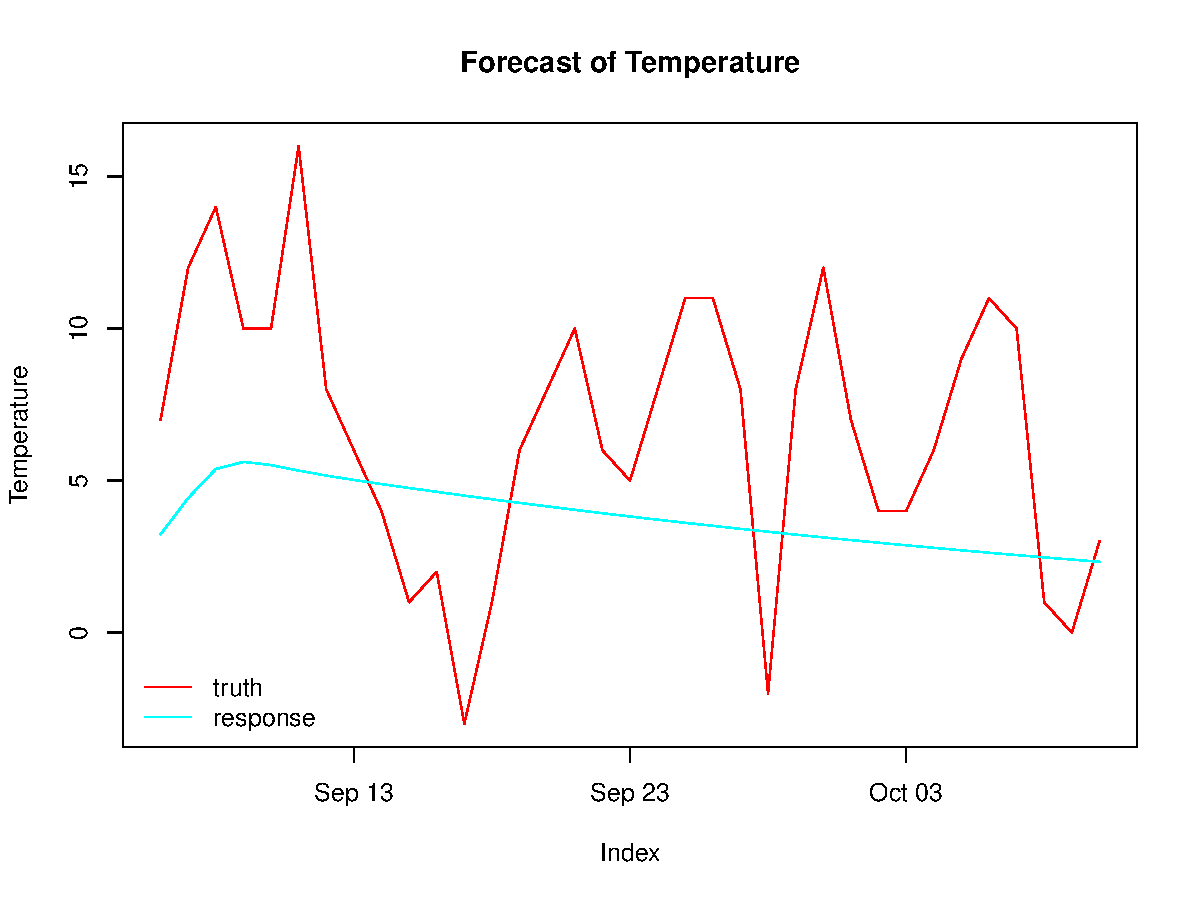
\includegraphics[width=\maxwidth]{figure/plotbatsTrain-1} 

}



\end{knitrout}
\doublespacing

Need to talk about results

Because the forecasts are only for the next 35 periods it's useful to be able to update the model continuously without retraining the model each time we want new forecasts. Univariate forecasting models in \pkg{mlr} can be updated using \code{updateModel()}. 

\singlespacing
\begin{knitrout}
\definecolor{shadecolor}{rgb}{0.969, 0.969, 0.969}\color{fgcolor}\begin{kframe}
\begin{alltt}
\hlstd{update.tbats} \hlkwb{=} \hlkwd{updateModel}\hlstd{(train.tbats, climate.task,} \hlkwc{newdata} \hlstd{= m4.test)}
\hlkwd{predict}\hlstd{(update.tbats,} \hlkwc{task} \hlstd{= climate.task)}
\end{alltt}
\begin{verbatim}
## Prediction: 35 observations
## predict.type: response
## threshold: 
## time: 0.00
##                     response
## 2009-09-04 23:59:54 6.319959
## 2009-09-05 23:59:48 7.875401
## 2009-09-06 23:59:43 8.209328
## 2009-09-07 23:59:37 8.157638
## 2009-09-08 23:59:31 8.083591
## 2009-09-09 23:59:26 8.055280
## ... (35 rows, 1 cols)
\end{verbatim}
\end{kframe}
\end{knitrout}
\doublespacing

\subsection{Multivariate Forecasting}

The package \pkg{BigVAR} has been implemented for multivariate forecasting. \pkg{BigVAR} allows for estimation of high dimensional time series through including structured Lasso penalties to the vector autoregression framework~\cite{bigvarpaper}. 

\singlespacing
\begin{knitrout}
\definecolor{shadecolor}{rgb}{0.969, 0.969, 0.969}\color{fgcolor}\begin{kframe}
\begin{alltt}
\hlstd{bigvar.mod} \hlkwb{=} \hlkwd{makeLearner}\hlstd{(}\hlstr{"mfcregr.BigVAR"}\hlstd{,}\hlkwc{p} \hlstd{=} \hlnum{25}\hlstd{,} \hlkwc{struct} \hlstd{=} \hlstr{"SparseLag"}\hlstd{,}
                         \hlkwc{gran} \hlstd{=} \hlkwd{c}\hlstd{(}\hlnum{50}\hlstd{,} \hlnum{60}\hlstd{),}\hlkwc{h} \hlstd{=} \hlnum{35}\hlstd{,} \hlkwc{n.ahead} \hlstd{=} \hlnum{35}\hlstd{)}
\end{alltt}
\end{kframe}
\end{knitrout}


\begin{knitrout}
\definecolor{shadecolor}{rgb}{0.969, 0.969, 0.969}\color{fgcolor}\begin{kframe}
\begin{alltt}
\hlstd{train.bigvar} \hlkwb{=} \hlkwd{train}\hlstd{(}\hlkwc{learner} \hlstd{= bigvar.mod,} \hlkwc{task} \hlstd{= mfcregr.all.task )}
\end{alltt}
\end{kframe}
\end{knitrout}

\begin{knitrout}
\definecolor{shadecolor}{rgb}{0.969, 0.969, 0.969}\color{fgcolor}\begin{kframe}
\begin{verbatim}
## Model for learner.id=mfcregr.BigVAR; learner.class=mfcregr.BigVAR
## Trained on: task.id = bigvar; obs = 1828; features = 0
## Hyperparameters: p=25,struct=SparseLag,gran=50,60,h=35,n.ahead=35
\end{verbatim}
\end{kframe}
\end{knitrout}
\doublespacing

Predictions for \code{multiForecast} methods have a similar output to \code{multiclass} methods, returning multiple truth and response variables. A multivariate version of MASE has been implimented which takes the mean of each MASE score for the individual variables.

\singlespacing
\begin{knitrout}
\definecolor{shadecolor}{rgb}{0.969, 0.969, 0.969}\color{fgcolor}\begin{kframe}
\begin{alltt}
\hlstd{predict.bigvar} \hlkwb{=} \hlkwd{predict}\hlstd{(train.bigvar,} \hlkwc{newdata} \hlstd{= eu.test)}
\hlstd{predict.bigvar}
\end{alltt}
\begin{verbatim}
## Prediction: 32 observations
## predict.type: response
## threshold: 
## time: 0.02
##                     truth.DAX truth.SMI truth.CAC truth.FTSE response.DAX
## 1998-07-12 07:50:46   5905.15    8047.3    4252.1     5960.2     5852.841
## 1998-07-13 17:32:18   5961.45    8099.0    4304.4     5988.4     5820.194
## 1998-07-15 03:13:50   5942.06    8166.0    4311.1     5990.3     5801.712
## 1998-07-16 12:55:23   5975.88    8160.0    4333.1     6003.4     5790.565
## 1998-07-17 22:36:55   6018.89    8227.2    4339.9     6009.6     5781.540
## 1998-07-19 08:18:27   6000.84    8205.0    4319.2     5969.7     5772.087
##                     response.SMI response.CAC response.FTSE
## 1998-07-12 07:50:46     7982.503     4192.149      5997.825
## 1998-07-13 17:32:18     7960.779     4153.550      6037.958
## 1998-07-15 03:13:50     7955.264     4130.674      6063.687
## 1998-07-16 12:55:23     7958.119     4115.612      6083.094
## 1998-07-17 22:36:55     7965.061     4103.302      6100.075
## 1998-07-19 08:18:27     7973.586     4091.154      6116.419
## ... (32 rows, 8 cols)
\end{verbatim}
\begin{alltt}
\hlkwd{performance}\hlstd{(predict.bigvar, multivar.mase,} \hlkwc{task} \hlstd{= mfcregr.all.task)}
\end{alltt}
\begin{verbatim}
## multivar.mase 
##     0.2209703
\end{verbatim}
\end{kframe}
\end{knitrout}

\begin{knitrout}
\definecolor{shadecolor}{rgb}{0.969, 0.969, 0.969}\color{fgcolor}

{\centering 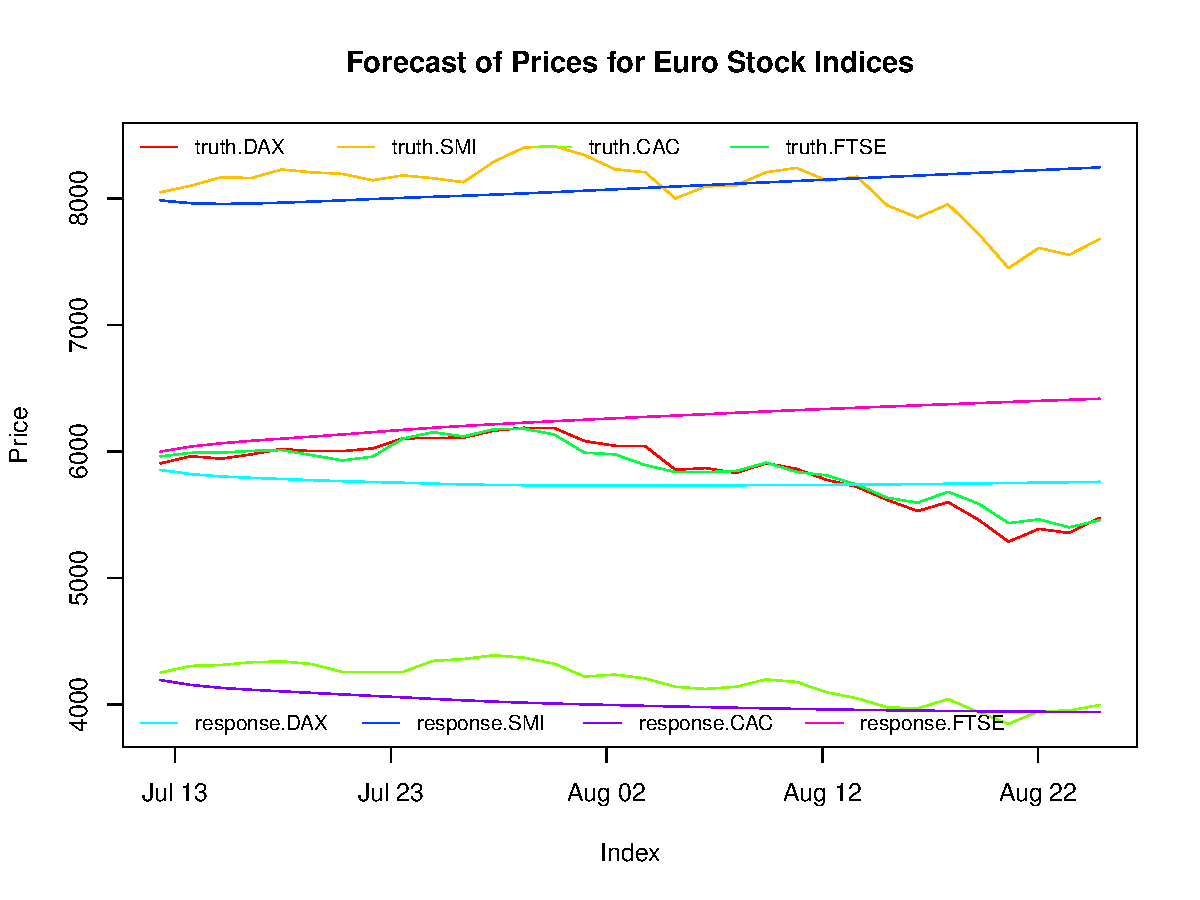
\includegraphics[width=\maxwidth]{figure/bigVarplot-1} 

}



\end{knitrout}
\doublespacing

\section{Resampling with Time}

While TBATS is one of the most well known time series models, the order selection process or the ARIMA errors and whether to include trend, damped trend, or seasonal periods can be a subjective process that makes finding the best model difficult for users. One of the first proposals for automated forecasting methods comes from ~\cite{hannanOrder} for automatic order selection of ARIMA models. Innovations are obtained by fitting high order autoregressive models to the data and then computing the likelihood of potential models through a series of standard regresssions. Proprietary algorithms from software such as \proglang{Forecast Pro} ~\cite{forecastpro} and \proglang{Autobox} ~\cite{reillyautobox} are well known and have performed to high standards in competitions such as the M3 forecasting competition ~\cite{Makridakis2000451}. One of the most well known R packages for automated forecast is \pkg{forecast} ~\cite{HyndForecast} which contains several methods for automated forecasting including exponential smoothing based methods and step-wise algorithms for forecasting with ARIMA models.

Forecasting in \pkg{mlr} takes a machine learning approach, creating a parameter set for a given model and using an optimization method to search over the parameter space. To do this, we will use a windowing resampling scheme to train over the possible models. Resampling schemes such as cross-validation, bootstrapping, etc. are common in machine learning for dealing with the bias-variance tradeoff ~\cite{Friedman1997} ~\cite{rodriguezkfold}. When their is a time component to the data, windowing schemes are useful in allowing a valid resampling scheme while still maintaining the time properties of the series. Figure one gives an example of fixed and growing windows. Given a horizon and initial starting point the window slides forward one step each time while either shifting in the fixed case or enlarging by one in the growing case. Growing and fixed window resampling such as from ~\cite{hyndman2014forecasting} are now available in the \code{resampling()} function of \pkg{mlr}. 

\begin{figure}[ht]
\caption{Resampling with a window scheme as exampled by caret ~\cite{windowingcaret}. The top graphs are fixed window cross validation while the bottom graphs are growing window cross validation. }
  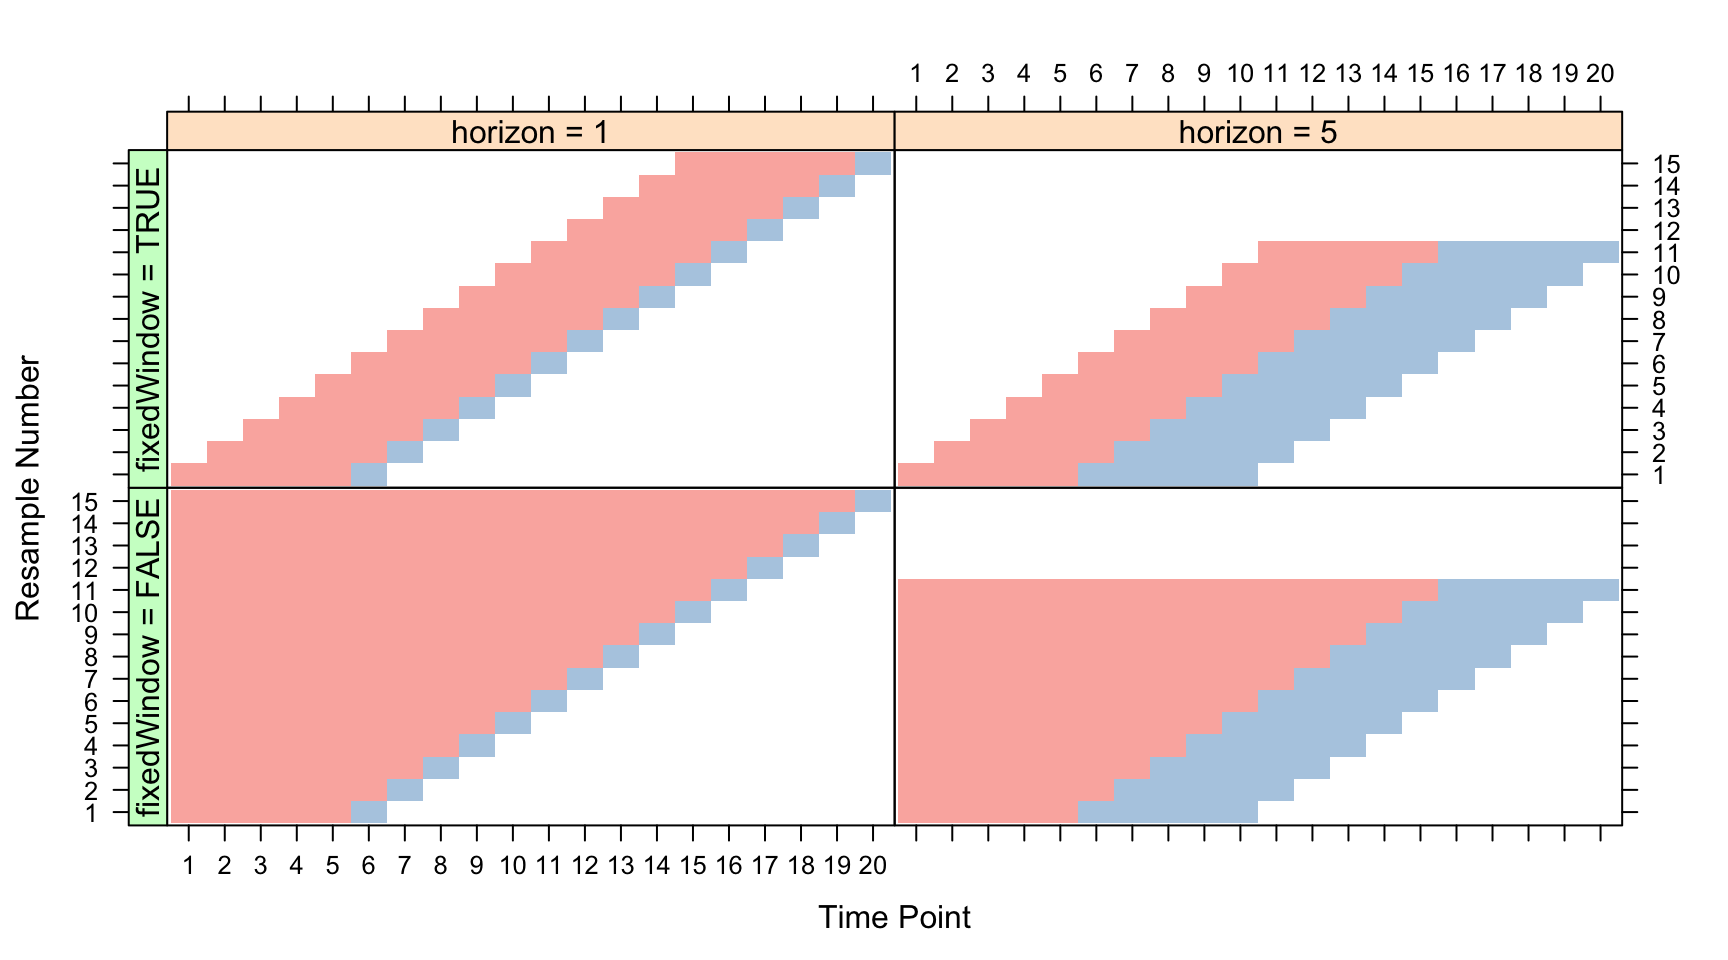
\includegraphics[scale = .23]{windowing_pic_caret}
  \centering
\end{figure}
%% Note: If there is markup in \(sub)section, then it has to be escape as above.
\newpage

A windowing resampling process is created in the function \code{makeResampleDesc()} by supplying the resampling type, horizon, initial window, the length of the series, and an optional argument to skip over some windows for the sake of time.

\singlespacing
\begin{knitrout}
\definecolor{shadecolor}{rgb}{0.969, 0.969, 0.969}\color{fgcolor}\begin{kframe}
\begin{alltt}
\hlstd{resampDesc} \hlkwb{=} \hlkwd{makeResampleDesc}\hlstd{(}\hlstr{"GrowingCV"}\hlstd{,} \hlkwc{horizon} \hlstd{=} \hlnum{35L}\hlstd{,}
                               \hlkwc{initial.window} \hlstd{=} \hlnum{.7}\hlstd{,}
                               \hlkwc{size} \hlstd{=} \hlkwd{nrow}\hlstd{(}\hlkwd{getTaskData}\hlstd{(climate.task)),}
                               \hlkwc{skip} \hlstd{=} \hlnum{.004}\hlstd{)}
\hlstd{resampDesc}
\end{alltt}
\begin{verbatim}
## Window description:
##  growing with 79 iterations:
##  448 observations in initial window and 35 horizon.
## Predict: test
## Stratification: FALSE
\end{verbatim}
\end{kframe}
\end{knitrout}
\doublespacing


To make a parameter set to tune over \pkg{mlr} uses \pkg{ParamHelpers} ~\cite{paramhelper}. There are several types of tools to help us search our parameter space including grid search, random search ~\cite{Bergstra}, to search our parameter space for the most optimal model.


\singlespacing                                      
\begin{knitrout}
\definecolor{shadecolor}{rgb}{0.969, 0.969, 0.969}\color{fgcolor}\begin{kframe}
\begin{alltt}
\hlstd{parSet} \hlkwb{=} \hlkwd{makeParamSet}\hlstd{(}
           \hlkwd{makeLogicalParam}\hlstd{(}\hlkwc{id} \hlstd{=} \hlstr{"use.box.cox"}\hlstd{,}\hlkwc{default} \hlstd{=} \hlnum{FALSE}\hlstd{,}
                            \hlkwc{tunable} \hlstd{=} \hlnum{TRUE}\hlstd{),}
           \hlkwd{makeLogicalParam}\hlstd{(}\hlkwc{id} \hlstd{=} \hlstr{"use.trend"}\hlstd{,} \hlkwc{default} \hlstd{=} \hlnum{FALSE}\hlstd{,}
                            \hlkwc{tunable} \hlstd{=} \hlnum{TRUE}\hlstd{),}
           \hlkwd{makeLogicalParam}\hlstd{(}\hlkwc{id} \hlstd{=} \hlstr{"use.damped.trend"}\hlstd{,} \hlkwc{default} \hlstd{=} \hlnum{FALSE}\hlstd{,}
                            \hlkwc{tunable} \hlstd{=} \hlnum{TRUE}\hlstd{),}
           \hlkwd{makeLogicalParam}\hlstd{(}\hlkwc{id} \hlstd{=} \hlstr{"seasonal.periods"}\hlstd{,} \hlkwc{default} \hlstd{=} \hlnum{FALSE}\hlstd{,}
                            \hlkwc{tunable} \hlstd{=} \hlnum{TRUE}\hlstd{),}
           \hlkwd{makeIntegerParam}\hlstd{(}\hlkwc{id} \hlstd{=} \hlstr{"max.p"}\hlstd{,} \hlkwc{upper} \hlstd{=} \hlnum{30}\hlstd{,} \hlkwc{lower} \hlstd{=} \hlnum{1}\hlstd{,}
                            \hlkwc{trafo} \hlstd{=} \hlkwa{function}\hlstd{(}\hlkwc{x}\hlstd{) x}\hlopt{*}\hlnum{2}\hlstd{),}
           \hlkwd{makeIntegerParam}\hlstd{(}\hlkwc{id} \hlstd{=} \hlstr{"start.p"}\hlstd{,} \hlkwc{upper} \hlstd{=} \hlnum{30}\hlstd{,} \hlkwc{lower} \hlstd{=} \hlnum{1}\hlstd{,}
                            \hlkwc{trafo} \hlstd{=} \hlkwa{function}\hlstd{(}\hlkwc{x}\hlstd{) x}\hlopt{*}\hlnum{2}\hlstd{),}
           \hlkwd{makeIntegerParam}\hlstd{(}\hlkwc{id} \hlstd{=} \hlstr{"max.q"}\hlstd{,} \hlkwc{upper} \hlstd{=} \hlnum{30}\hlstd{,} \hlkwc{lower} \hlstd{=} \hlnum{1}\hlstd{,}
                            \hlkwc{trafo} \hlstd{=} \hlkwa{function}\hlstd{(}\hlkwc{x}\hlstd{) x}\hlopt{*}\hlnum{2}\hlstd{),}
           \hlkwd{makeIntegerParam}\hlstd{(}\hlkwc{id} \hlstd{=} \hlstr{"start.q"}\hlstd{,} \hlkwc{upper} \hlstd{=} \hlnum{5}\hlstd{,} \hlkwc{lower} \hlstd{=} \hlnum{0}\hlstd{,}
                            \hlkwc{trafo} \hlstd{=} \hlkwa{function}\hlstd{(}\hlkwc{x}\hlstd{) x}\hlopt{*}\hlnum{2}\hlstd{),}
           \hlkwd{makeIntegerParam}\hlstd{(}\hlstr{"max.P"}\hlstd{,} \hlkwc{lower} \hlstd{=} \hlnum{0}\hlstd{,} \hlkwc{upper} \hlstd{=} \hlnum{5}\hlstd{),}
           \hlkwd{makeIntegerParam}\hlstd{(}\hlstr{"max.Q"}\hlstd{,} \hlkwc{lower} \hlstd{=} \hlnum{0}\hlstd{,} \hlkwc{upper} \hlstd{=} \hlnum{5}\hlstd{),}
           \hlkwd{makeDiscreteParam}\hlstd{(}\hlstr{"ic"}\hlstd{,}\hlkwc{values} \hlstd{=} \hlkwd{c}\hlstd{(}\hlstr{"aicc"}\hlstd{,}\hlstr{"aic"}\hlstd{,}\hlstr{"bic"}\hlstd{)),}
           \hlkwd{makeDiscreteParam}\hlstd{(}\hlstr{"test"}\hlstd{,}\hlkwc{values} \hlstd{=} \hlkwd{c}\hlstd{(}\hlstr{"kpss"}\hlstd{,}\hlstr{"adf"}\hlstd{,}\hlstr{"pp"}\hlstd{)),}
           \hlkwd{makeDiscreteParam}\hlstd{(}\hlstr{"seasonal.test"}\hlstd{,}
                            \hlkwc{values} \hlstd{=} \hlkwd{c}\hlstd{(}\hlstr{"ocsb"}\hlstd{,} \hlstr{"ch"}\hlstd{)),}
          \hlkwd{makeLogicalParam}\hlstd{(}\hlstr{"biasadj"}\hlstd{,} \hlkwc{default} \hlstd{=} \hlnum{FALSE}\hlstd{)}
        \hlstd{)}

\hlcom{#Specify tune by grid estimation}
\hlstd{ctrl} \hlkwb{=} \hlkwd{makeTuneControlIrace}\hlstd{(}\hlkwc{maxExperiments} \hlstd{=} \hlnum{500L}\hlstd{)}
\end{alltt}
\end{kframe}
\end{knitrout}
\doublespacing

Using \code{tuneParams()} the model is tuned for the task using the specified resampling scheme, parameter set, tune control, and measure. The \code{trafo} argument allows the tuning process to take values on a seperate scale than the one described. In the tuning scheme above, trafo will look search over $1, 4, 9, ..., 81$, and $100$ values of lag, selecting the model with the best lag structure. For this tuning task we use MASE ~\cite{Hyndman2006} as a measure of performance \footnote{Models with a seasonal difference $> 0$ may be favorably biased as we use the non-seasonal MASE score}.

\singlespacing
\begin{knitrout}
\definecolor{shadecolor}{rgb}{0.969, 0.969, 0.969}\color{fgcolor}\begin{kframe}
\begin{alltt}
\hlcom{#}
\hlkwd{library}\hlstd{(}\hlstr{"parallelMap"}\hlstd{)}
\hlkwd{parallelStartSocket}\hlstd{(}\hlnum{8}\hlstd{)}
\hlkwd{configureMlr}\hlstd{(}\hlkwc{on.learner.error} \hlstd{=} \hlstr{"warn"}\hlstd{)}
\hlkwd{set.seed}\hlstd{(}\hlnum{1234}\hlstd{)}
\hlstd{tbatsTune} \hlkwb{=} \hlkwd{tuneParams}\hlstd{(}\hlkwd{makeLearner}\hlstd{(}\hlstr{"fcregr.tbats"}\hlstd{,} \hlkwc{h} \hlstd{=} \hlnum{35}\hlstd{),}
                       \hlkwc{task} \hlstd{= climate.task,} \hlkwc{resampling} \hlstd{= resampDesc,}
                       \hlkwc{par.set} \hlstd{= parSet,} \hlkwc{control} \hlstd{= ctrl,} \hlkwc{measures} \hlstd{= mase)}
\hlkwd{parallelStop}\hlstd{()}
\hlstd{tbatsTune}\hlopt{$}\hlstd{y}
\end{alltt}
\end{kframe}
\end{knitrout}

\begin{knitrout}
\definecolor{shadecolor}{rgb}{0.969, 0.969, 0.969}\color{fgcolor}\begin{kframe}
\begin{verbatim}
## mase.test.mean 
##     0.06877628
\end{verbatim}
\end{kframe}
\end{knitrout}

Using \pkg{mlr}'s built in plotting routines the tuning parameters can be analyzed graphically using partial dependence plots ~\ref{partialdep}. Because of constraints which do not allow logical types in the partial dependence plots, the below code takes all of the logical parameters from \code{tbatsTune} and coerces them to numeric.

\begin{knitrout}
\definecolor{shadecolor}{rgb}{0.969, 0.969, 0.969}\color{fgcolor}

{\centering 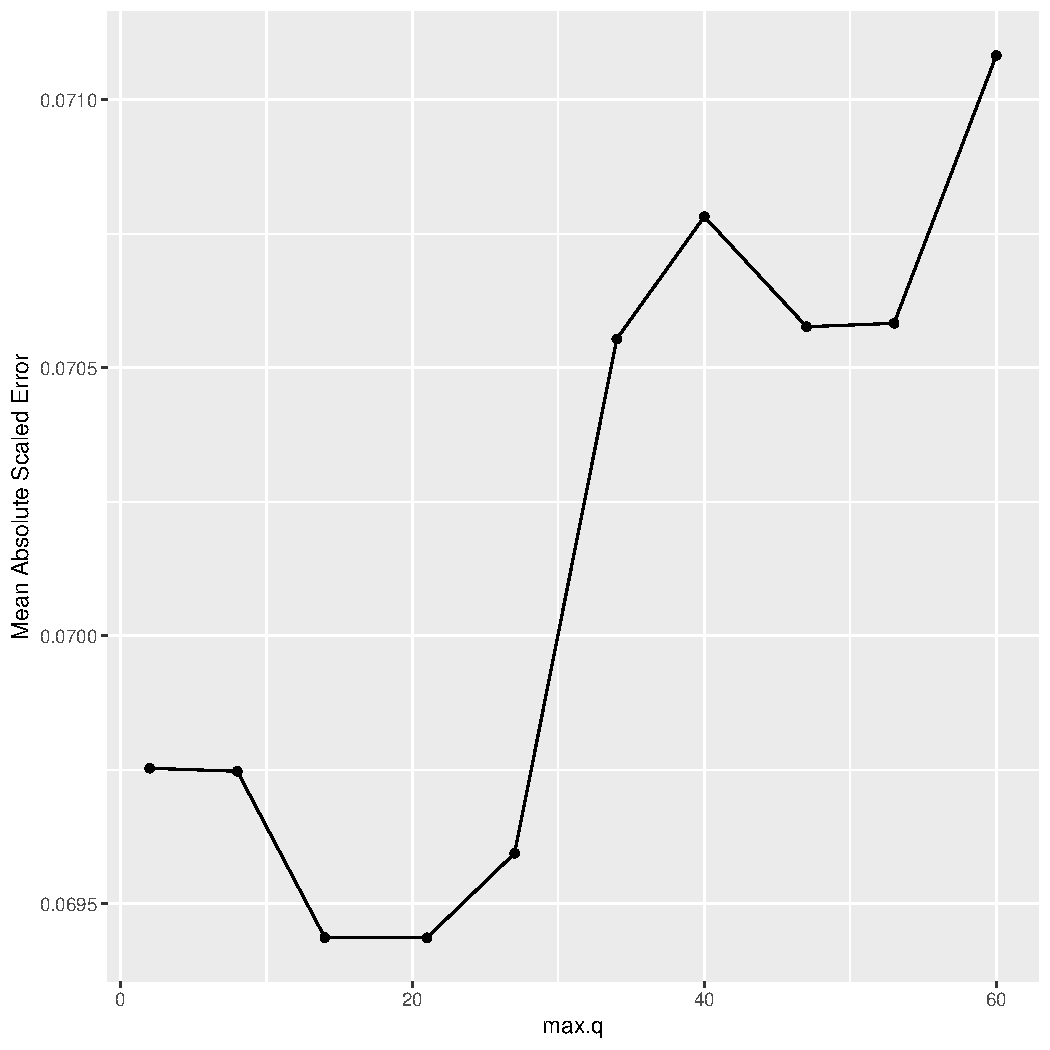
\includegraphics[width=\maxwidth]{figure/loadTuneTbats2-1} 

}



\end{knitrout}
\doublespacing

For this model the best maximum number of moving average coefficients is two. The best model's parameters are extracted using \code{setHyperPars()} and passed to \code{train()} to go over the full data set.

\singlespacing
\begin{knitrout}
\definecolor{shadecolor}{rgb}{0.969, 0.969, 0.969}\color{fgcolor}\begin{kframe}
\begin{alltt}
\hlstd{lrn} \hlkwb{=} \hlkwd{setHyperPars}\hlstd{(}\hlkwd{makeLearner}\hlstd{(}\hlstr{"fcregr.tbats"}\hlstd{,} \hlkwc{h} \hlstd{=} \hlnum{35}\hlstd{),}
                   \hlkwc{par.vals} \hlstd{= tbatsTune}\hlopt{$}\hlstd{x)}
\hlstd{m} \hlkwb{=} \hlkwd{train}\hlstd{(lrn, climate.task)}
\end{alltt}
\end{kframe}
\end{knitrout}
\doublespacing

To make predictions for our test set we simply pass our model, task, and test data to \code{predict()}

\singlespacing
\begin{knitrout}
\definecolor{shadecolor}{rgb}{0.969, 0.969, 0.969}\color{fgcolor}\begin{kframe}
\begin{alltt}
\hlstd{climate.pred} \hlkwb{=} \hlkwd{predict}\hlstd{(m,} \hlkwc{newdata} \hlstd{= m4.test)}
\hlkwd{performance}\hlstd{(climate.pred,} \hlkwc{measures} \hlstd{= mase,} \hlkwc{task} \hlstd{= climate.task)}
\end{alltt}
\begin{verbatim}
##       mase 
## 0.06145902
\end{verbatim}
\end{kframe}
\end{knitrout}
\doublespacing

For comparison, TBATS is run in \pkg{forecast} with it's base parameters

\singlespacing
\begin{knitrout}
\definecolor{shadecolor}{rgb}{0.969, 0.969, 0.969}\color{fgcolor}\begin{kframe}
\begin{alltt}
\hlkwd{library}\hlstd{(forecast)}
\hlstd{forecast.train.tbats} \hlkwb{=} \hlkwd{tbats}\hlstd{(}\hlkwd{ts}\hlstd{(m4.train,}\hlkwc{frequency} \hlstd{=} \hlnum{365}\hlstd{))}
\hlstd{forecast.tbats} \hlkwb{=} \hlkwd{forecast}\hlstd{(forecast.train.tbats,}\hlkwc{h}\hlstd{=}\hlnum{35}\hlstd{)}
\hlcom{# Calculate MASE}
\hlkwd{sum}\hlstd{(}\hlkwd{abs}\hlstd{(}\hlkwd{coredata}\hlstd{(m4.test)}\hlopt{-}\hlstd{forecast.tbats}\hlopt{$}\hlstd{mean))} \hlopt{/}
 \hlstd{((}\hlkwd{nrow}\hlstd{(m4.test)} \hlopt{/} \hlstd{(}\hlkwd{nrow}\hlstd{(m4.test)} \hlopt{+} \hlnum{1}\hlstd{))} \hlopt{*}
     \hlkwd{sum}\hlstd{(}\hlkwd{abs}\hlstd{(}\hlkwd{diff}\hlstd{(}\hlkwd{coredata}\hlstd{(m4.test)))))}
\end{alltt}
\begin{verbatim}
## [1] 1.951852
\end{verbatim}
\end{kframe}
\end{knitrout}
\doublespacing

Now it's possible to see the clear benefit of the forecast extension to \pkg{mlr}. While \pkg{forecast} does some automated tuning, this model would still require extensive manual testing in an attempt to find the best model. By automating this process we come to a faster solution with minimal work.

\begin{knitrout}
\definecolor{shadecolor}{rgb}{0.969, 0.969, 0.969}\color{fgcolor}
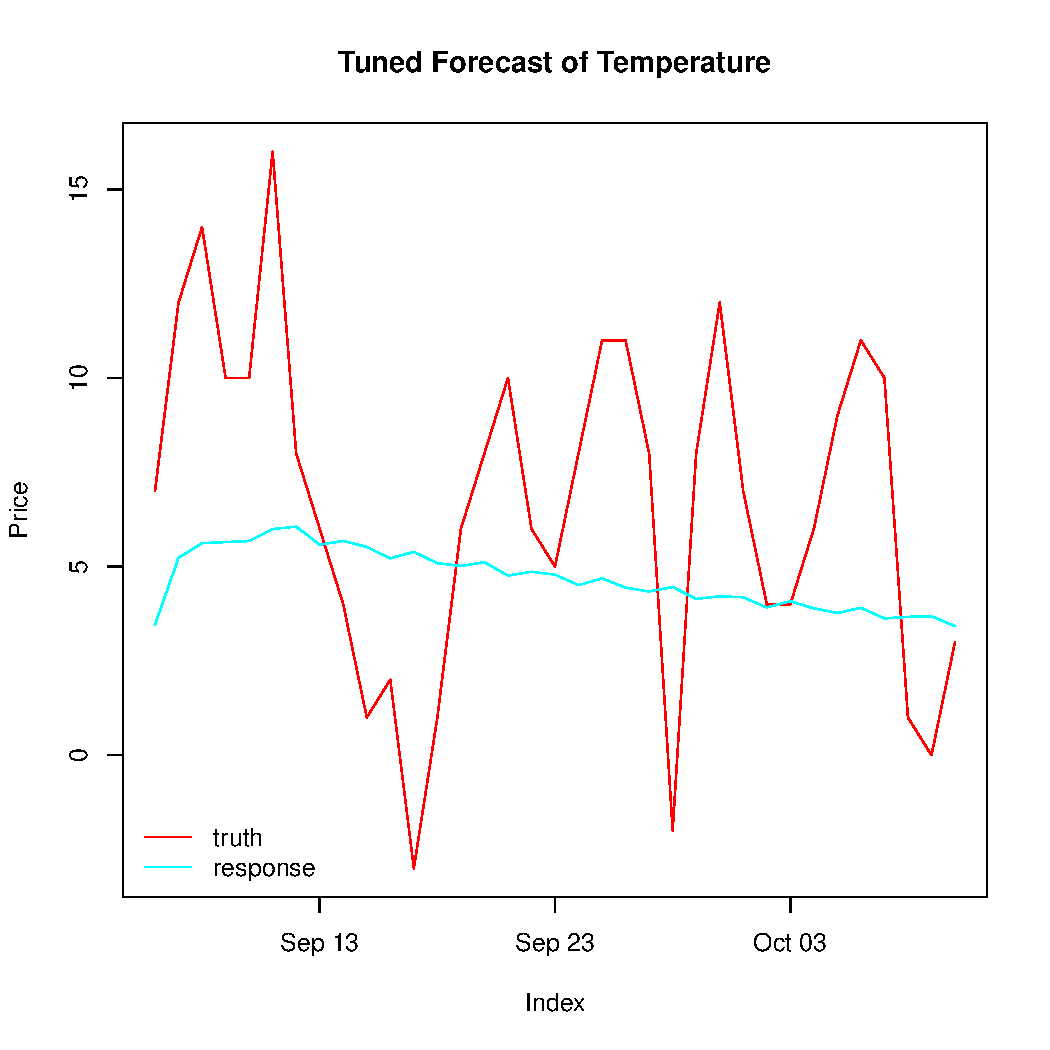
\includegraphics[width=\maxwidth]{figure/plottbatsTune-1} 

\end{knitrout}

To this author's knowledge, this is the first package in \proglang{R} that allows for automated tuning and training of GARCH models ~\cite{garchengels}. It is possible to pass and train multiple types of GARCH models while also tuning the models respective parameters. In this example we also use \code{predict.type = "quantile"} to estimate confidence intervals for the forecast.

\singlespacing
\begin{knitrout}
\definecolor{shadecolor}{rgb}{0.969, 0.969, 0.969}\color{fgcolor}\begin{kframe}
\begin{alltt}
\hlstd{par_set} \hlkwb{=} \hlkwd{makeParamSet}\hlstd{(}
  \hlkwd{makeDiscreteParam}\hlstd{(}\hlkwc{id} \hlstd{=} \hlstr{"model"}\hlstd{,} \hlkwc{values} \hlstd{=} \hlkwd{c}\hlstd{(}\hlstr{"sGARCH"}\hlstd{,} \hlstr{"csGARCH"}\hlstd{)),}
  \hlkwd{makeIntegerVectorParam}\hlstd{(}\hlkwc{id} \hlstd{=} \hlstr{"garchOrder"}\hlstd{,} \hlkwc{len} \hlstd{=} \hlnum{2L}\hlstd{,} \hlkwc{lower} \hlstd{=} \hlkwd{c}\hlstd{(}\hlnum{1}\hlstd{,}\hlnum{1}\hlstd{),}
                         \hlkwc{upper} \hlstd{=} \hlkwd{c}\hlstd{(}\hlnum{4}\hlstd{,}\hlnum{4}\hlstd{)),}
  \hlkwd{makeIntegerVectorParam}\hlstd{(}\hlkwc{id} \hlstd{=} \hlstr{"armaOrder"}\hlstd{,} \hlkwc{len} \hlstd{=} \hlnum{2L}\hlstd{,} \hlkwc{lower} \hlstd{=} \hlkwd{c}\hlstd{(}\hlnum{5}\hlstd{,}\hlnum{1}\hlstd{),}
                         \hlkwc{upper} \hlstd{=} \hlkwd{c}\hlstd{(}\hlnum{8}\hlstd{,}\hlnum{3}\hlstd{)),}
  \hlkwd{makeLogicalParam}\hlstd{(}\hlkwc{id} \hlstd{=} \hlstr{"include.mean"}\hlstd{),}
  \hlkwd{makeLogicalParam}\hlstd{(}\hlkwc{id} \hlstd{=} \hlstr{"archm"}\hlstd{),}
  \hlkwd{makeDiscreteParam}\hlstd{(}\hlkwc{id} \hlstd{=} \hlstr{"distribution.model"}\hlstd{,}
                    \hlkwc{values} \hlstd{=} \hlkwd{c}\hlstd{(}\hlstr{"norm"}\hlstd{,}\hlstr{"std"}\hlstd{,}\hlstr{"jsu"}\hlstd{)),}
  \hlkwd{makeDiscreteParam}\hlstd{(}\hlkwc{id} \hlstd{=} \hlstr{"stationarity"}\hlstd{,} \hlkwd{c}\hlstd{(}\hlnum{0}\hlstd{,}\hlnum{1}\hlstd{)),}
  \hlkwd{makeDiscreteParam}\hlstd{(}\hlkwc{id} \hlstd{=} \hlstr{"fixed.se"}\hlstd{,} \hlkwd{c}\hlstd{(}\hlnum{0}\hlstd{,}\hlnum{1}\hlstd{)),}
  \hlkwd{makeDiscreteParam}\hlstd{(}\hlkwc{id} \hlstd{=} \hlstr{"solver"}\hlstd{,} \hlkwc{values} \hlstd{=} \hlstr{"nloptr"}\hlstd{)}
\hlstd{)}

\hlcom{#Specify tune by grid estimation}
\hlstd{ctrl} \hlkwb{=} \hlkwd{makeTuneControlIrace}\hlstd{(}\hlkwc{maxExperiments} \hlstd{=} \hlnum{400L}\hlstd{)}

\hlkwd{parallelStartSocket}\hlstd{(}\hlnum{6}\hlstd{)}
\hlkwd{configureMlr}\hlstd{(}\hlkwc{on.learner.error} \hlstd{=} \hlstr{"warn"}\hlstd{)}
\hlkwd{set.seed}\hlstd{(}\hlnum{1234}\hlstd{)}
\hlstd{garchTune} \hlkwb{=} \hlkwd{tuneParams}\hlstd{(}\hlkwd{makeLearner}\hlstd{(}\hlstr{"fcregr.garch"}\hlstd{,} \hlkwc{n.ahead}\hlstd{=} \hlnum{35}\hlstd{),}
                       \hlkwc{task} \hlstd{= climate.task,} \hlkwc{resampling} \hlstd{= resampDesc,}
                       \hlkwc{par.set} \hlstd{= par_set,} \hlkwc{control} \hlstd{= ctrl,}
                       \hlkwc{measures} \hlstd{= mase)}
\hlkwd{parallelStop}\hlstd{()}
\hlstd{garchTune}\hlopt{$}\hlstd{y}
\end{alltt}
\end{kframe}
\end{knitrout}
\doublespacing

\begin{knitrout}
\definecolor{shadecolor}{rgb}{0.969, 0.969, 0.969}\color{fgcolor}\begin{kframe}
\begin{verbatim}
## mase.test.mean 
##     0.07888857
\end{verbatim}
\end{kframe}
\end{knitrout}


Because the partial dependence plots are still in development they do not work well with \code{makeNumericVectorParams()} such as \code{garchOrder} and \code{armaOrder}. Instead of looking at each $p,q$ individually, we simply sum them and look at the maximum coefficient values for the $p,q$ order of the GARCH component and the ARMA component.

\singlespacing
\begin{knitrout}
\definecolor{shadecolor}{rgb}{0.969, 0.969, 0.969}\color{fgcolor}\begin{kframe}
\begin{alltt}
\hlstd{garch.hyperpar} \hlkwb{=} \hlkwd{generateHyperParsEffectData}\hlstd{(garchTune,}
                    \hlkwc{trafo} \hlstd{=} \hlnum{TRUE}\hlstd{,} \hlkwc{include.diagnostics} \hlstd{=} \hlnum{FALSE}\hlstd{,}
                    \hlkwc{partial.dep} \hlstd{=} \hlnum{TRUE}\hlstd{)}
\hlstd{garch.hyperpar}\hlopt{$}\hlstd{data} \hlkwb{=} \hlstd{garch.hyperpar}\hlopt{$}\hlstd{data[}
                      \hlopt{-}\hlkwd{which}\hlstd{(garch.hyperpar}\hlopt{$}\hlstd{data}\hlopt{$}\hlstd{mase.test.mean} \hlopt{==}
                            \hlkwd{max}\hlstd{(garch.hyperpar}\hlopt{$}\hlstd{data}\hlopt{$}\hlstd{mase.test.mean)),]}
\hlstd{garch.hyperpar}\hlopt{$}\hlstd{data}\hlopt{$}\hlstd{garchOrder1} \hlkwb{=} \hlstd{garch.hyperpar}\hlopt{$}\hlstd{data}\hlopt{$}\hlstd{garchOrder1} \hlopt{+}
                                  \hlstd{garch.hyperpar}\hlopt{$}\hlstd{data}\hlopt{$}\hlstd{garchOrder2}
\hlstd{garch.hyperpar}\hlopt{$}\hlstd{data}\hlopt{$}\hlstd{garchOrder2} \hlkwb{=} \hlkwa{NULL}
\hlkwd{colnames}\hlstd{(garch.hyperpar}\hlopt{$}\hlstd{data)[}\hlnum{2}\hlstd{]} \hlkwb{=} \hlstr{"garchOrder"}
\hlstd{garch.hyperpar}\hlopt{$}\hlstd{data}\hlopt{$}\hlstd{armaOrder1} \hlkwb{=} \hlstd{garch.hyperpar}\hlopt{$}\hlstd{data}\hlopt{$}\hlstd{armaOrder1} \hlopt{+}
                                 \hlstd{garch.hyperpar}\hlopt{$}\hlstd{data}\hlopt{$}\hlstd{armaOrder2}
\hlstd{garch.hyperpar}\hlopt{$}\hlstd{data}\hlopt{$}\hlstd{armaOrder2} \hlkwb{=} \hlkwa{NULL}
\hlkwd{colnames}\hlstd{(garch.hyperpar}\hlopt{$}\hlstd{data)[}\hlnum{3}\hlstd{]} \hlkwb{=} \hlstr{"armaOrder"}
\hlstd{garch.hyperpar}\hlopt{$}\hlstd{data}\hlopt{$}\hlstd{include.mean} \hlkwb{=} \hlkwd{as.numeric}\hlstd{(garch.hyperpar}\hlopt{$}\hlstd{data}\hlopt{$}\hlstd{include.mean)}
\hlstd{garch.hyperpar}\hlopt{$}\hlstd{data}\hlopt{$}\hlstd{archm} \hlkwb{=} \hlkwd{as.numeric}\hlstd{(garch.hyperpar}\hlopt{$}\hlstd{data}\hlopt{$}\hlstd{archm)}
\hlkwd{plotHyperParsEffect}\hlstd{(garch.hyperpar,} \hlkwc{x}\hlstd{=} \hlstr{"garchOrder"}\hlstd{,} \hlkwc{y} \hlstd{=} \hlstr{"mase.test.mean"}\hlstd{,}
                     \hlkwc{plot.type} \hlstd{=} \hlstr{"line"}\hlstd{,}
                     \hlkwc{partial.dep.learn} \hlstd{=} \hlstr{"regr.randomForest"}\hlstd{)}
\end{alltt}
\end{kframe}
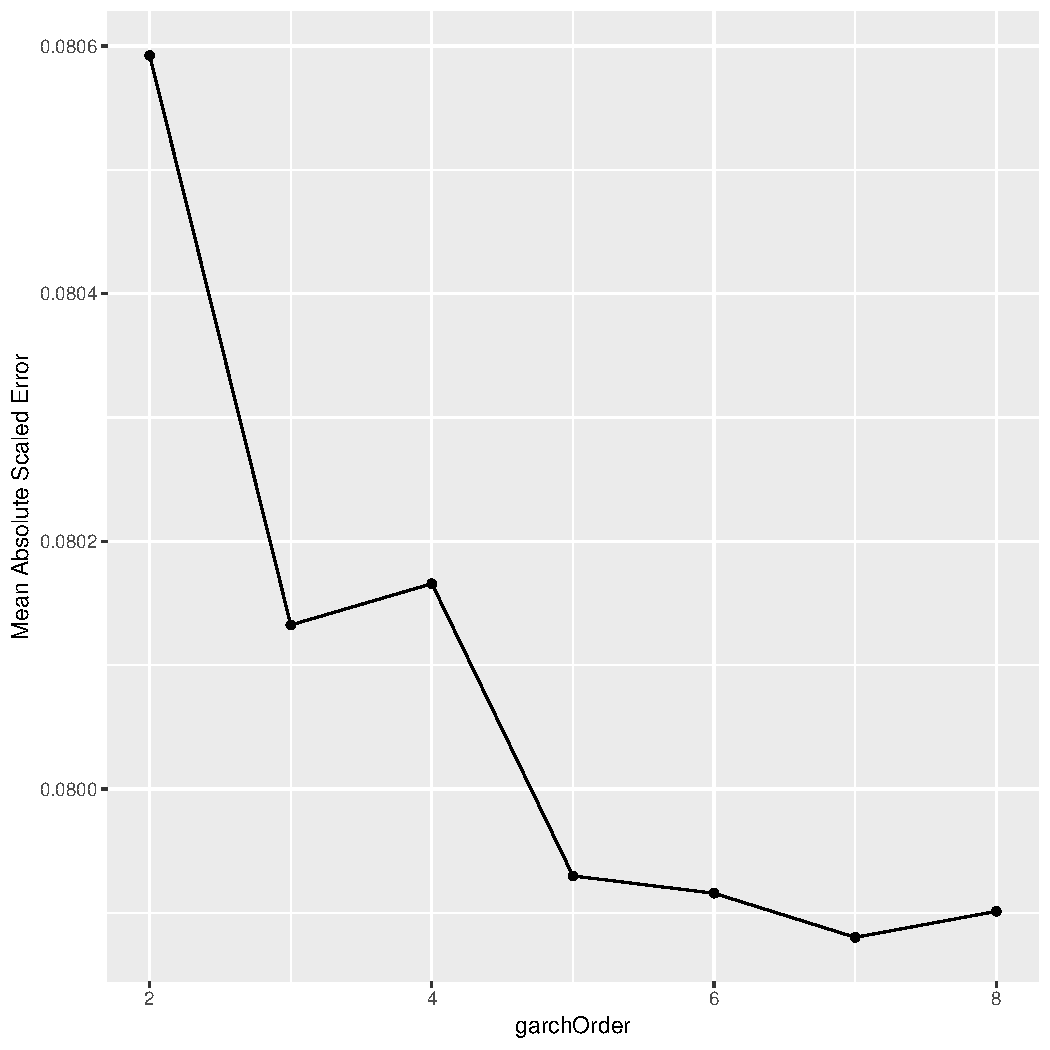
\includegraphics[width=\maxwidth]{figure/makeHyperPlot-1} 
\begin{kframe}\begin{alltt}
\hlkwd{plotHyperParsEffect}\hlstd{(garch.hyperpar,} \hlkwc{x}\hlstd{=} \hlstr{"armaOrder"}\hlstd{,} \hlkwc{y} \hlstd{=} \hlstr{"mase.test.mean"}\hlstd{,}
                     \hlkwc{plot.type} \hlstd{=} \hlstr{"line"}\hlstd{,}
                     \hlkwc{partial.dep.learn} \hlstd{=} \hlstr{"regr.randomForest"}\hlstd{)}
\end{alltt}
\end{kframe}
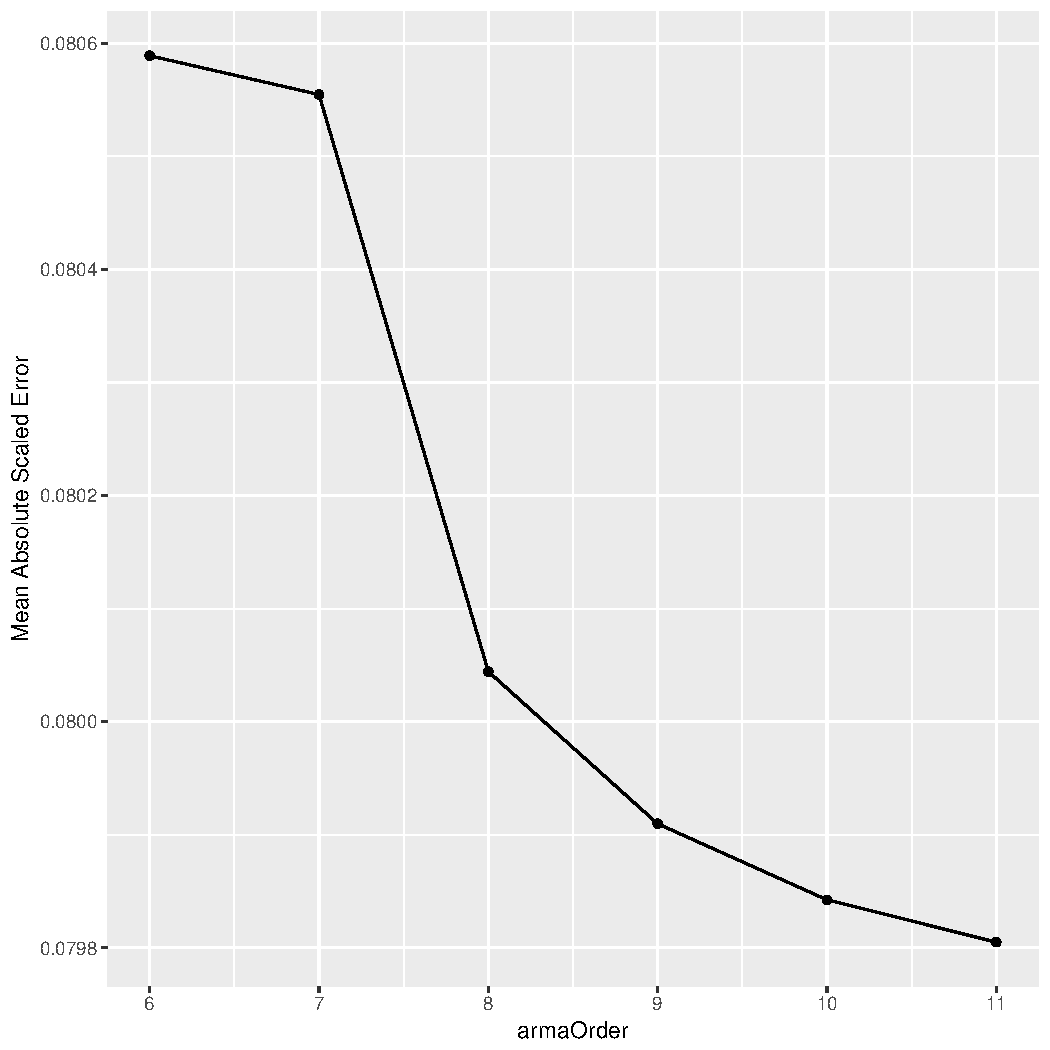
\includegraphics[width=\maxwidth]{figure/makeHyperPlot-2} 

\end{knitrout}
\doublespacing

The dependence plots show that for both the GARCH and ARMA orders, as the order is increased, the MASE score decreases. We would most likely find a better model if we allowed the order of the model to increase up to around fifteen or twenty or both. Forecasting models with quantiles are treated the same as any other learner post-tuning. The best hyperparameters are taken and a final model is trained over the entire dataset.

\singlespacing
\begin{knitrout}
\definecolor{shadecolor}{rgb}{0.969, 0.969, 0.969}\color{fgcolor}\begin{kframe}
\begin{alltt}
\hlstd{tuned.lrn} \hlkwb{=} \hlkwd{setHyperPars}\hlstd{(}\hlkwd{makeLearner}\hlstd{(}\hlstr{"fcregr.garch"}\hlstd{,}
                                     \hlkwc{predict.type} \hlstd{=} \hlstr{"quantile"}\hlstd{),}
                         \hlkwc{par.vals} \hlstd{= garchTune}\hlopt{$}\hlstd{x)}
\hlstd{garch.train} \hlkwb{=} \hlkwd{train}\hlstd{(tuned.lrn, climate.task)}
\end{alltt}
\end{kframe}
\end{knitrout}



\begin{knitrout}
\definecolor{shadecolor}{rgb}{0.969, 0.969, 0.969}\color{fgcolor}\begin{kframe}
\begin{alltt}
\hlstd{climate.pred} \hlkwb{=} \hlkwd{predict}\hlstd{(garch.train,} \hlkwc{newdata} \hlstd{= m4.test)}
\hlstd{climate.pred}
\end{alltt}
\begin{verbatim}
## Prediction: 35 observations
## predict.type: quantile
## threshold: 
## time: 0.01
##            truth response se.quantile0.05 se.quantile0.95
## 2009-09-06     7 3.870648      -2.8377519        10.57905
## 2009-09-07    12 5.940932      -0.7674667        12.64933
## 2009-09-08    14 6.962520       0.1060161        13.81902
## 2009-09-09    10 7.336334       0.3367573        14.33591
## 2009-09-10    10 7.473346       0.4736223        14.47307
## 2009-09-11    16 7.737601       0.7377337        14.73747
## ... (35 rows, 4 cols)
\end{verbatim}
\begin{alltt}
\hlkwd{performance}\hlstd{(climate.pred,} \hlkwc{measures} \hlstd{= mase,} \hlkwc{task} \hlstd{= climate.task)}
\end{alltt}
\begin{verbatim}
##       mase 
## 0.05589035
\end{verbatim}
\end{kframe}
\end{knitrout}

\begin{knitrout}
\definecolor{shadecolor}{rgb}{0.969, 0.969, 0.969}\color{fgcolor}
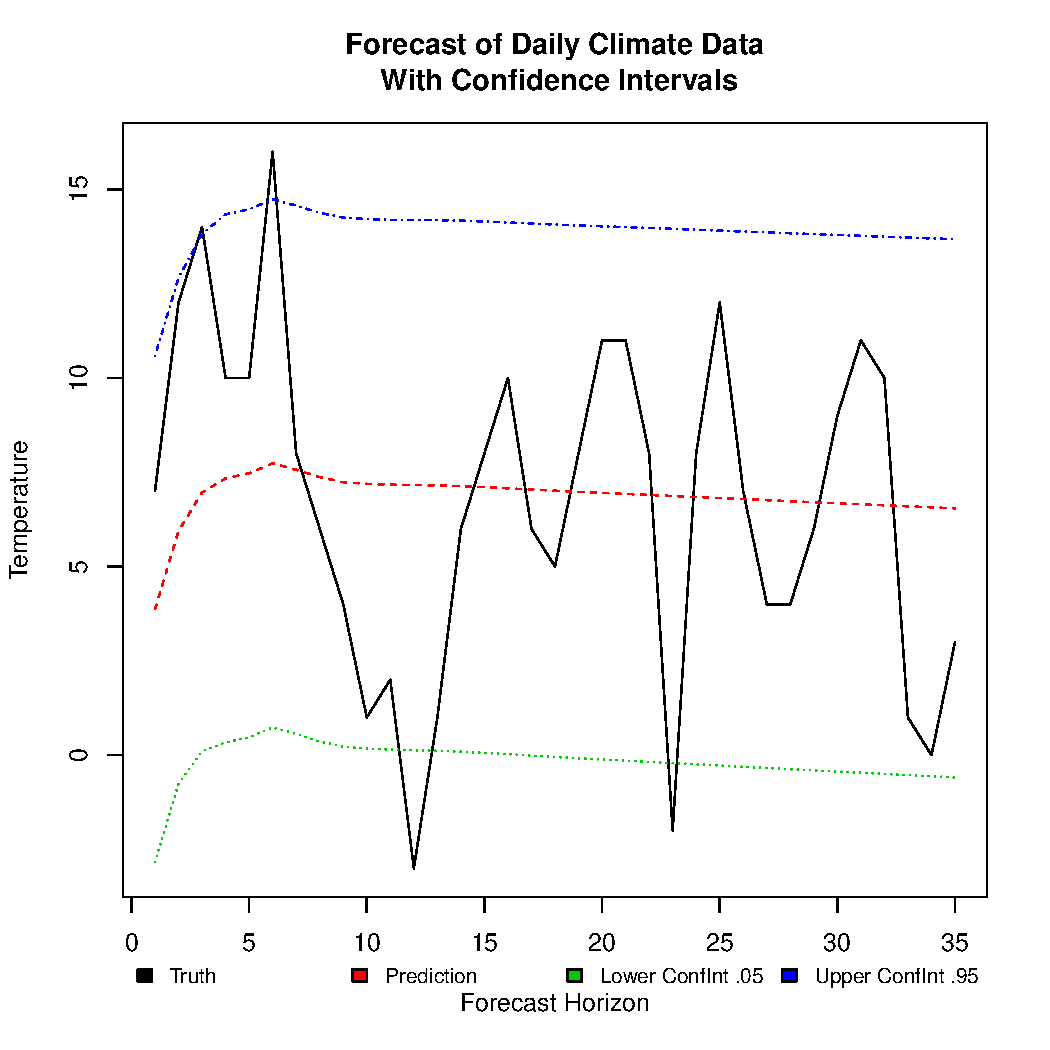
\includegraphics[width=\maxwidth]{figure/trainGarchTuned4-1} 

\end{knitrout}
\doublespacing

The simple model here performs relatively well. The extremes of the test data are almost all within the given bounds of the 95\% confidence interval. With a bit more tuning and perhaps an alternative control for the search over the parameter space, the reader would easily find a better model. While GARCH is excellent at catching the conditional heteroskedasticity of the past series, the TBATS model performs well in terms of catching long or multiseasonal type periods. Section~\ref{sub:stackedUnivar} goes over how to combine forecasting models to make benefit of both models of their strengths.


\section{Forecasting with Machine Learning Models}

\subsection{Forecasting with Regression Tasks}

The forecasting extension of \pkg{mlr} includes a preprocessing function that allows supervised machine learning models. the function \code{createLagDiffFeatures()} allows for $AR(p,d)$ structures to be imbedded in machine learning models.
\singlespacing
\begin{knitrout}
\definecolor{shadecolor}{rgb}{0.969, 0.969, 0.969}\color{fgcolor}\begin{kframe}
\begin{alltt}
\hlstd{climate.regr.task} \hlkwb{=} \hlkwd{makeRegrTask}\hlstd{(}\hlkwc{id} \hlstd{=} \hlstr{"lagged gbm"}\hlstd{,}
                                 \hlkwc{data} \hlstd{=} \hlkwd{as.data.frame}\hlstd{(m4.train),}
                                 \hlkwc{target} \hlstd{=} \hlstr{"target_var"}\hlstd{)}
\hlstd{climate.task.lag} \hlkwb{=} \hlkwd{createLagDiffFeatures}\hlstd{(climate.regr.task,}
                                         \hlkwc{lag} \hlstd{=} \hlnum{1L}\hlopt{:}\hlnum{24L}\hlstd{,}
                                         \hlkwc{difference} \hlstd{=} \hlnum{1L}\hlstd{,}
                                         \hlkwc{na.pad}\hlstd{=}\hlnum{FALSE}\hlstd{)}
\hlstd{climate.task.lag}
\end{alltt}
\begin{verbatim}
## Supervised task: lagged gbm
## Type: regr
## Target: target_var
## Observations: 615
## Features:
## numerics  factors  ordered 
##       24        0        0 
## Missings: FALSE
## Has weights: FALSE
## Has blocking: FALSE
\end{verbatim}
\end{kframe}
\end{knitrout}
\doublespacing

Notice that \code{createLagDiffFeatures()} returns a new task with the lagged variables as the new features. Once the lagged task is created the model is trained or tuned like any other.

\singlespacing
\begin{knitrout}
\definecolor{shadecolor}{rgb}{0.969, 0.969, 0.969}\color{fgcolor}\begin{kframe}
\begin{alltt}
\hlstd{lag.gbm} \hlkwb{=} \hlkwd{makeLearner}\hlstd{(}\hlstr{"regr.gbm"}\hlstd{,} \hlkwc{par.vals} \hlstd{=} \hlkwd{list}\hlstd{(}\hlkwc{n.trees} \hlstd{=} \hlnum{20000}\hlstd{,}
                                                  \hlkwc{shrinkage} \hlstd{=} \hlnum{.000001}\hlstd{,}
                                                  \hlkwc{interaction.depth} \hlstd{=} \hlnum{15}\hlstd{,}
                                                  \hlkwc{bag.fraction} \hlstd{=} \hlnum{.7}\hlstd{))}
\hlstd{gbm.train} \hlkwb{=} \hlkwd{train}\hlstd{(lag.gbm, climate.task.lag)}
\end{alltt}
\end{kframe}
\end{knitrout}
\doublespacing

The \code{forecast()} function allows machine learning models to do arbitary n-step ahead forecasts. Let the one step ahead forecast be defined by

\begin{equation}
\hat{y}_{t+1} = \sum_{i=1}^p \left(\rho_i \Delta_d y_{i} + \epsilon_{i}\right)
\end{equation}
where $\rho_i$ is the autoregressiver parameter of order $p$ and $d$ is the lag of the difference operator $\Delta$. Then the $n$-step ahead forecast is defined as

\begin{equation}
\hat{y}_{t+n} = \sum_{i=t+1}^{n} \left(\rho_i \Delta_d \hat{y}_{i} + \epsilon_{i}\right)
\end{equation}


\singlespacing
\begin{knitrout}
\definecolor{shadecolor}{rgb}{0.969, 0.969, 0.969}\color{fgcolor}\begin{kframe}
\begin{alltt}
\hlstd{gbm.forecast} \hlkwb{=} \hlkwd{forecast}\hlstd{(gbm.train,} \hlkwc{h} \hlstd{=} \hlnum{35L}\hlstd{,}
                        \hlkwc{newdata} \hlstd{=} \hlkwd{as.data.frame}\hlstd{(m4.test))}
\hlkwd{performance}\hlstd{(gbm.forecast,mase,climate.task.lag)}
\end{alltt}
\end{kframe}
\end{knitrout}
\begin{knitrout}
\definecolor{shadecolor}{rgb}{0.969, 0.969, 0.969}\color{fgcolor}\begin{kframe}
\begin{verbatim}
## Prediction: 35 observations
## predict.type: response
## threshold: 
## time: 7.30
##   truth response
## 1     7 7.655469
## 2    12 8.234003
## 3    14 8.234003
## 4    10 8.234003
## 5    10 8.234003
## 6    16 8.234003
## ... (35 rows, 2 cols)
##      mase 
## 0.0558791
\end{verbatim}
\end{kframe}
\end{knitrout}

\doublespacing

\begin{knitrout}
\definecolor{shadecolor}{rgb}{0.969, 0.969, 0.969}\color{fgcolor}
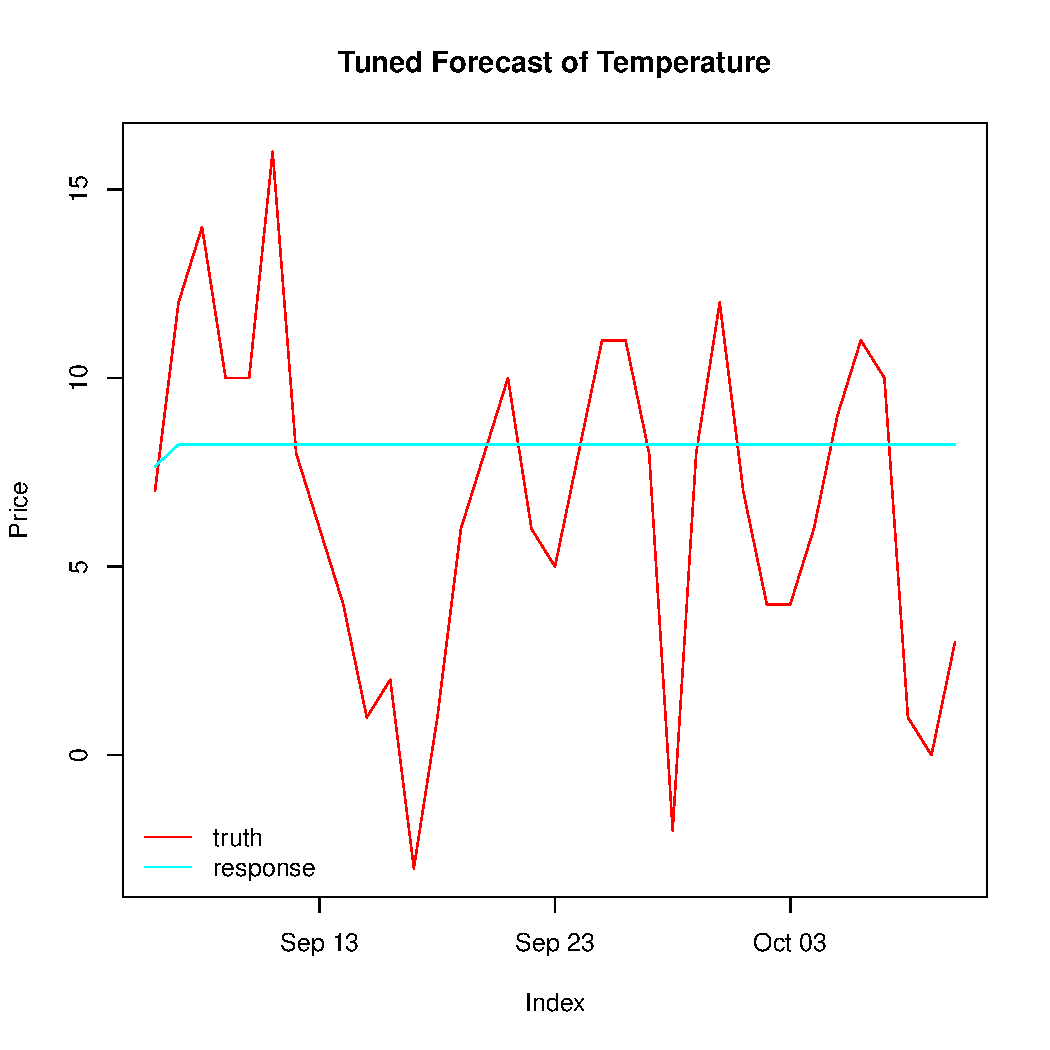
\includegraphics[width=\maxwidth]{figure/forecastgbmplot-1} 

\end{knitrout}

\subsection{Forecasting with Classification Tasks}

Forecasting for binary or multiclass outcomes~\cite{forecastBinary} is a common problem in the real world. However, research in this area of forecasting only started picking up speed in the last decade~\cite{ElliotBinary}. With a this new extension to \pkg{mlr} researchers now have the ability to take all the classification models in \pkg{mlr} and apply them to the forecasting context. For developing trading strategies, we normally have a discrete set of choices such as to buy, sell, or hold onto a stock. Using forecasting in mlr we can now train classification models that forecast these choices~\cite{foreclassif}. To example this, a simple buy, sell, or hold trading strategy will be built Using the \code{EuStockMarkets}'s DAX index. If the stock goes up by 5\% in a day we will buy, down 5\% we will sell, and otherwise we will hold onto the current stocks we have. 

\singlespacing
\begin{knitrout}
\definecolor{shadecolor}{rgb}{0.969, 0.969, 0.969}\color{fgcolor}\begin{kframe}
\begin{alltt}
\hlstd{DAX} \hlkwb{=} \hlstd{EuStockMarkets}\hlopt{$}\hlstd{DAX}\hlopt{/}\hlkwd{lag}\hlstd{(EuStockMarkets}\hlopt{$}\hlstd{DAX,}
                             \hlnum{7}\hlstd{,}\hlkwc{nap.pad} \hlstd{=} \hlnum{FALSE}\hlstd{)} \hlopt{-} \hlnum{1}
\hlstd{trade.strat} \hlkwb{=} \hlkwd{ifelse}\hlstd{(DAX} \hlopt{>} \hlnum{.05}\hlstd{,} \hlstr{"Buy"}\hlstd{,}
                     \hlkwd{ifelse}\hlstd{(DAX} \hlopt{< -}\hlnum{.05}\hlstd{,} \hlstr{"Sell"}\hlstd{,} \hlstr{"Hold"}\hlstd{))}
\hlstd{trade.strat} \hlkwb{=} \hlstd{trade.strat[}\hlnum{8}\hlopt{:}\hlnum{1860}\hlstd{]}
\hlstd{euro.classif.data} \hlkwb{=} \hlkwd{data.frame}\hlstd{(}\hlkwc{trade.strat} \hlstd{= trade.strat ,}
                               \hlkwc{row.names} \hlstd{=} \hlkwd{index}\hlstd{(trade.strat))}
\hlcom{# Note: Error on multiples of the same observation}
\hlstd{euro.classif.train} \hlkwb{=} \hlstd{euro.classif.data[}\hlnum{1}\hlopt{:}\hlnum{1838}\hlstd{,,}\hlkwc{drop} \hlstd{=} \hlnum{FALSE}\hlstd{]}
\hlstd{euro.classif.test}  \hlkwb{=} \hlstd{euro.classif.data[}\hlnum{1839}\hlopt{:}\hlnum{1853}\hlstd{,,}\hlkwc{drop} \hlstd{=} \hlnum{FALSE}\hlstd{]}
\hlstd{classif.task} \hlkwb{=} \hlkwd{makeClassifTask}\hlstd{(}\hlkwc{data} \hlstd{= euro.classif.train,}
                               \hlkwc{target} \hlstd{=} \hlstr{"DAX"}\hlstd{)}
\hlstd{classif.task.lag} \hlkwb{=} \hlkwd{createLagDiffFeatures}\hlstd{(classif.task,}
                                         \hlkwc{lag} \hlstd{=} \hlnum{1L}\hlopt{:}\hlnum{565L}\hlstd{,}
                                         \hlkwc{na.pad} \hlstd{=} \hlnum{FALSE}\hlstd{)}
\hlstd{classif.learn} \hlkwb{=} \hlkwd{makeLearner}\hlstd{(}\hlstr{"classif.boosting"}\hlstd{,} \hlkwc{xval} \hlstd{=} \hlnum{1}\hlstd{,}
                            \hlkwc{mfinal} \hlstd{=} \hlnum{200}\hlstd{,} \hlkwc{minsplit} \hlstd{=} \hlnum{10}\hlstd{)}
\end{alltt}
\end{kframe}
\end{knitrout}

\begin{knitrout}
\definecolor{shadecolor}{rgb}{0.969, 0.969, 0.969}\color{fgcolor}\begin{kframe}
\begin{alltt}
\hlstd{classif.train} \hlkwb{=} \hlkwd{train}\hlstd{(classif.learn, classif.task.lag)}
\hlstd{classif.fc} \hlkwb{=} \hlkwd{forecast}\hlstd{(classif.train,} \hlkwc{h}\hlstd{=}\hlnum{15}\hlstd{,} \hlkwc{newdata} \hlstd{= euro.classif.test)}
\hlkwd{performance}\hlstd{(classif.fc)}
\end{alltt}
\end{kframe}
\end{knitrout}



\begin{knitrout}
\definecolor{shadecolor}{rgb}{0.969, 0.969, 0.969}\color{fgcolor}\begin{kframe}
\begin{verbatim}
## Prediction: 15 observations
## predict.type: response
## threshold: 
## time: 422.87
##   truth response
## 1  Hold     Hold
## 2  Hold     Hold
## 3  Sell     Hold
## 4  Hold     Hold
## 5  Hold     Hold
## 6  Hold     Hold
## ... (15 rows, 2 cols)
##      mmce 
## 0.4666667
\end{verbatim}
\end{kframe}
\end{knitrout}
\doublespacing

With the models and methedologies available in \pkg{mlr}, forecasting binary outcomes is now as simple as any other model. These tools can be used for further research in areas such as directions of stock movement~\cite{markClassifStock} and forecasting extreme values ~\cite{Chen2015UsingEV}. 

\section{Lambert W Transforms}

Many machine learning and time series models rely one the assumption that our data or errors fit a normal distribution. This assumption becomes precarious when modeling the asymmetric and fat-tailed data of the real world. Lambert W Transforms are a family of generalized skewed distributions ~\cite{LambertGeneral} that have bijecetive and parametric functions that allow heavy tailed and asymettric data to appear more Gaussian  ~\cite{GaussLam}. 

Let $U$ be a continuous random variable with cdf $F_U(u|\beta)$ and pdf $f_U(u|\beta)$ given $\beta$ is a parameter vector. Define a continuous location-scale random variable $X\sim F_X(x|\beta)$. A locaton-scale skewed Lambert $W\times F_X$ random variable is defined as 
\begin{equation}
test %Z = U\exp\left(\frac{\delta}{2}(U^2)^\right),\; \delta\ge 0
\end{equation}
And the heavy-tailed Lambert $W\times F_X$ random variable can be defined as
\begin{equation}
test %Z = U\exp\left(\frac{\delta}{2}(U^2)^\alpha\right),\; \delta\ge 0\; \alpha > 0
\end{equation}

Given that $U = (X-\mu_X)/\sigma_X$ where $\mu_X$, $\sigma_X$, $\delta$, and $\alpha$ are the mean and standard deviation of X and the parameters to control skewness and asymetry , respectively. When $\delta = 0$, equation 12 reduces to a standard normal distribution. Equation 12 is the general form of Tukey's $h$ distribution ~\cite{ghdist} and the basis for Morgenthaler and Tukey's ~\cite{hhdist} skewed, heavy tailed family of $hh$ random variables.

\begin{equation}
  Z = \begin{cases}
               U\exp\left(\frac{\delta_l}{2}(U^2)^\alpha_l\right),\; \delta_l \ge 0\; \alpha_l > 0\\
               U\exp\left(\frac{\delta_r}{2}(U^2)^\alpha_r\right),\; \delta_r \ge 0 \alpha_r > 0
            \end{cases}
\end{equation}

\singlespacing
\begin{knitrout}
\definecolor{shadecolor}{rgb}{0.969, 0.969, 0.969}\color{fgcolor}
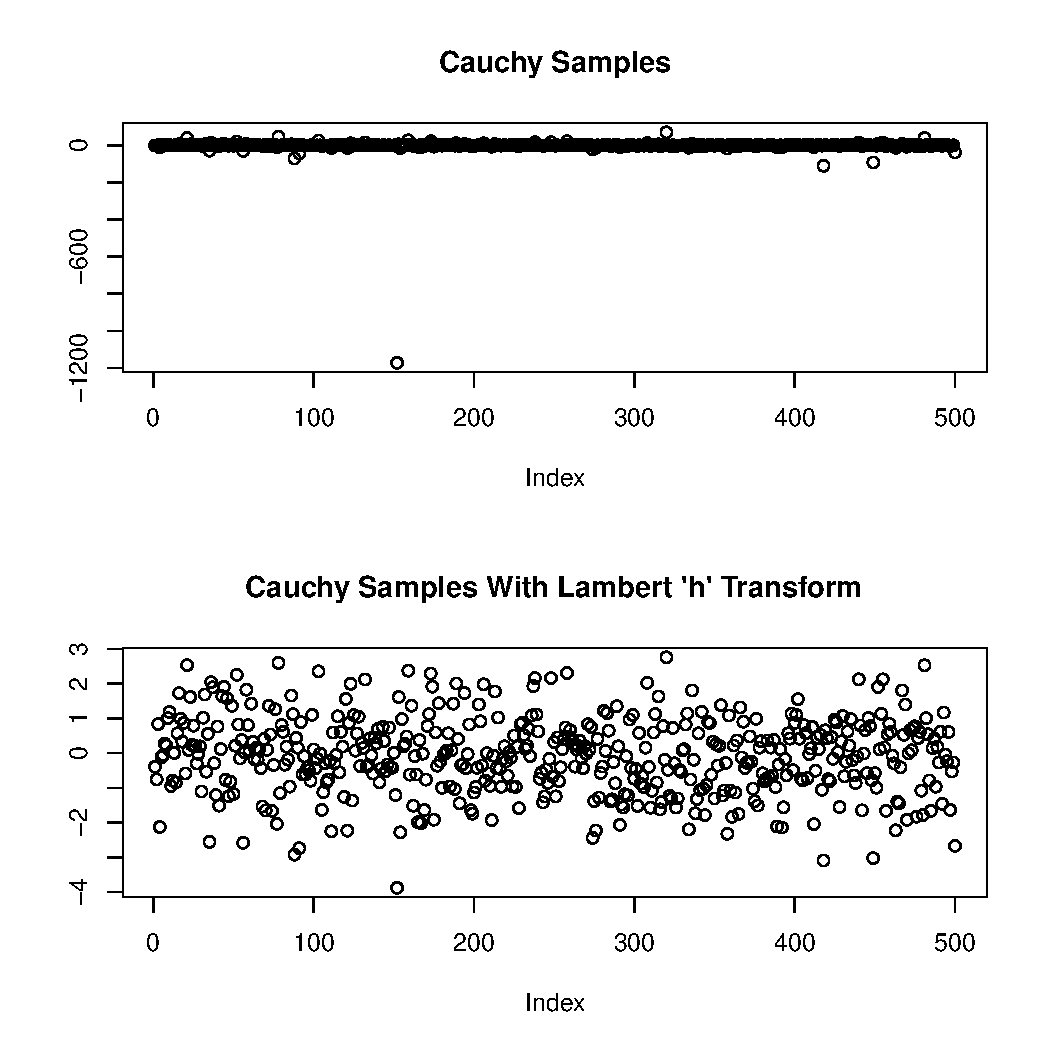
\includegraphics[width=\maxwidth]{figure/lambertWplots-1} 

\end{knitrout}
\doublespacing

The function \code{Gaussianize} is available in the package \pkg{LambertW} and has been made into a preprocessing function in \pkg{mlr}. Instead of calling \code{makeLearner()} to create a model, the function \code{makePreprocWrapperLambert()} can be used to create the model. Wrapping the model in this way allows the pre-processing function to be intertwined with the model itself. There are opportunities for users to accidentally bias there own results due to improperly applying pre-processing schemes. For instance, if a user demeaned their entire data set and then split the data into train and test subsets, the training data will be biased because demeaning the model over both the train and test data gives the training data information about the mean of the test data. What should happen instead is, the user first splits the data into training and test data, and then demeans each seperatly. But than what about cross-validation? The goal of cross-validation follows the above schema as well and it is very easy for a user, who assumes they have made a good faith attempt to not bias their model, will end up with overconfident results. Making the preprocessing part of the model itself allows \pkg{mlr} to overcome this. 

There will be a step for the training data or subset, for example to demean it, and then there will be a function for prediction on the testing data, or in the example above to demean the test set alone. In the context of Lambert W$\times$ F$()$ transforms, the $h$, $hh$, or $s$ distribution that gaussianizes the data is estimated from the training data. Then the estimated parameter values from the training set are used during prediction to gaussianize the test observations. The code below follows this methedology, creating the model with Lambert preprocessing, training the model, and then performing prediction. The end result to the user appears the same, but a significant amount of bias is reduced in the background.

\singlespacing
\begin{knitrout}
\definecolor{shadecolor}{rgb}{0.969, 0.969, 0.969}\color{fgcolor}\begin{kframe}
\begin{alltt}
\hlcom{# Need to make this more dramatic}
\hlstd{lamb.lrn} \hlkwb{=} \hlkwd{makePreprocWrapperLambert}\hlstd{(}\hlstr{"classif.lda"}\hlstd{,} \hlkwc{type} \hlstd{=} \hlstr{"h"}\hlstd{)}
\hlstd{lamb.lrn}
\end{alltt}
\begin{verbatim}
## Learner classif.lda.preproc from package MASS
## Type: classif
## Name: ; Short name: 
## Class: PreprocWrapperLambert
## Properties: numerics,factors,prob,twoclass,multiclass
## Predict-Type: response
## Hyperparameters: type=h,methods=IGMM,verbose=FALSE
\end{verbatim}
\begin{alltt}
\hlstd{lamb.trn} \hlkwb{=} \hlkwd{train}\hlstd{(lamb.lrn,iris.task,} \hlkwc{subset} \hlstd{=} \hlnum{1}\hlopt{:}\hlnum{120}\hlstd{)}
\hlstd{lamb.pred} \hlkwb{=} \hlkwd{predict}\hlstd{(lamb.trn, iris.task,} \hlkwc{subset} \hlstd{=} \hlnum{121}\hlopt{:}\hlnum{150}\hlstd{)}

\hlcom{# Do the non-LW version}
\hlstd{trn} \hlkwb{=} \hlkwd{train}\hlstd{(}\hlkwd{makeLearner}\hlstd{(}\hlstr{"classif.lda"}\hlstd{),iris.task,} \hlkwc{subset} \hlstd{=} \hlnum{1}\hlopt{:}\hlnum{120}\hlstd{)}
\hlstd{pred} \hlkwb{=} \hlkwd{predict}\hlstd{(trn, iris.task,} \hlkwc{subset} \hlstd{=} \hlnum{121}\hlopt{:}\hlnum{150}\hlstd{)}
\hlkwd{performance}\hlstd{(lamb.pred)}
\end{alltt}
\begin{verbatim}
## mmce 
##  0.1
\end{verbatim}
\begin{alltt}
\hlkwd{performance}\hlstd{(pred)}
\end{alltt}
\begin{verbatim}
## mmce 
##  0.1
\end{verbatim}
\end{kframe}
\end{knitrout}
\doublespacing

\section{Stacking Forecasting Learners}

Stacking is a form of ensemble learning~\cite{ensembleOverview} in which a learning algorithm is trained on the predictions of several other learning algorithms. Let $y_{i,m}$ be the prediction at time $i$ of model $m$. Given an aggregation function $\phi$, a stacked forecast learner~\cite{combineForecast} is represented as

\begin{equation}
\tilde{y}_{i+1} = \phi(\tilde{y}_{i+1,1}, \tilde{y}_{i+1,2},\dots, \tilde{y}_{i+1,m}, \sum_{j=1}^m \epsilon_{i+1,j})
\label{eq:ensemble}
\end{equation}

For a simple $\phi$ such as the ensemble average then equation~\ref{eq:ensemble} becomes

\begin{equation}
\tilde{y}_{i+1} = \frac{\tilde{y}_{i+1,1}, \tilde{y}_{i+1,2},\dots, \tilde{y}_{i+1,m}}{m}
\label{eq:ensembleAverage}
\end{equation}

In section~\ref{sub:stackedUnivar} the simple model average is used to show how stacked forecast models are built in \pkg{mlr}. Section~\ref{sub:multiStack} does a more advanced method of ensemble averaging involving the forecast of endogeneous variables.

\subsection{Stacking Univariate Learners}
\label{sub:stackedUnivar}

For this example the models TBATS, GARCH, and ARFIMA~\cite{arfima} are stacked together and averaged on the climate task data. A resample description is made, and the function \code{makeLearners()} is used to start multiple learners at the same time.

\singlespacing
\begin{knitrout}
\definecolor{shadecolor}{rgb}{0.969, 0.969, 0.969}\color{fgcolor}\begin{kframe}
\begin{alltt}
\hlstd{resamp.sub} \hlkwb{=} \hlkwd{makeResampleDesc}\hlstd{(}\hlstr{"GrowingCV"}\hlstd{,}
                          \hlkwc{horizon} \hlstd{=} \hlnum{35L}\hlstd{,}
                          \hlkwc{initial.window} \hlstd{=} \hlnum{.90}\hlstd{,}
                          \hlkwc{size} \hlstd{=} \hlkwd{nrow}\hlstd{(}\hlkwd{getTaskData}\hlstd{(climate.task)),}
                          \hlkwc{skip} \hlstd{=} \hlnum{.01}
                          \hlstd{)}
\hlstd{lrns} \hlkwb{=} \hlkwd{makeLearners}\hlstd{(}\hlkwd{c}\hlstd{(}\hlstr{"fcregr.tbats"}\hlstd{,}\hlstr{"fcregr.garch"}\hlstd{,}
                      \hlstr{"fcregr.arfima"}\hlstd{))}
\end{alltt}
\end{kframe}
\end{knitrout}
\doublespacing

The function \code{makeStackedLearner()} takes the initialized learners and sets the meta information for stacking. This method uses simple model averaging such as~\ref{eq:ensembleAveraging}, however a super learner~\cite{Wolpert92stackedgeneralization} can be used here, where $\phi()$ becomes another machine learning model.

\singlespacing
\begin{knitrout}
\definecolor{shadecolor}{rgb}{0.969, 0.969, 0.969}\color{fgcolor}\begin{kframe}
\begin{alltt}
\hlstd{stack.forecast} \hlkwb{=} \hlkwd{makeStackedLearner}\hlstd{(}\hlkwc{base.learners} \hlstd{= lrns,}
                       \hlkwc{predict.type} \hlstd{=} \hlstr{"response"}\hlstd{,}
                       \hlkwc{method} \hlstd{=} \hlstr{"average"}\hlstd{)}
\end{alltt}
\end{kframe}
\end{knitrout}
\doublespacing

Each of the stacked learners are tuned over the cross product of all model parameters. This leads to a change in design where, given that some models may have the same argument names, the full name of the model is placed before the argument. This leads to longer code, but tuning over the cross product of the models allows for a more honest perspective of how each model interacts in the stack.

\singlespacing
\begin{knitrout}
\definecolor{shadecolor}{rgb}{0.969, 0.969, 0.969}\color{fgcolor}\begin{kframe}
\begin{alltt}
\hlcom{# Simple param set for tuning sub learners}
\hlstd{ps} \hlkwb{=} \hlkwd{makeParamSet}\hlstd{(}
  \hlkwd{makeDiscreteParam}\hlstd{(}\hlstr{"fcregr.tbats.h"}\hlstd{,} \hlkwc{values} \hlstd{=} \hlnum{35}\hlstd{),}
  \hlkwd{makeDiscreteParam}\hlstd{(}\hlstr{"fcregr.garch.n.ahead"}\hlstd{,} \hlkwc{values} \hlstd{=} \hlnum{35}\hlstd{),}
  \hlkwd{makeDiscreteParam}\hlstd{(}\hlstr{"fcregr.arfima.h"}\hlstd{,} \hlkwc{values} \hlstd{=} \hlnum{35}\hlstd{),}
  \hlkwd{makeDiscreteParam}\hlstd{(}\hlstr{"fcregr.arfima.estim"}\hlstd{,} \hlkwc{values} \hlstd{=} \hlstr{"ls"}\hlstd{),}
  \hlkwd{makeDiscreteParam}\hlstd{(}\hlkwc{id} \hlstd{=} \hlstr{"fcregr.garch.model"}\hlstd{,}
                    \hlkwc{values} \hlstd{=} \hlkwd{c}\hlstd{(}\hlstr{"csGARCH"}\hlstd{)),}
  \hlkwd{makeIntegerVectorParam}\hlstd{(}\hlkwc{id} \hlstd{=} \hlstr{"fcregr.garch.garchOrder"}\hlstd{,}
                         \hlkwc{len} \hlstd{=} \hlnum{2L}\hlstd{,} \hlkwc{lower} \hlstd{=} \hlkwd{c}\hlstd{(}\hlnum{1}\hlstd{),}
                         \hlkwc{upper} \hlstd{=} \hlkwd{c}\hlstd{(}\hlnum{6}\hlstd{)),}
  \hlkwd{makeIntegerVectorParam}\hlstd{(}\hlkwc{id} \hlstd{=} \hlstr{"fcregr.garch.armaOrder"}\hlstd{,}
                         \hlkwc{len} \hlstd{=} \hlnum{2L}\hlstd{,} \hlkwc{lower} \hlstd{=} \hlkwd{c}\hlstd{(}\hlnum{1}\hlstd{),}
                         \hlkwc{upper} \hlstd{=} \hlkwd{c}\hlstd{(}\hlnum{4}\hlstd{)),}
  \hlkwd{makeDiscreteParam}\hlstd{(}\hlkwc{id} \hlstd{=} \hlstr{"fcregr.garch.distribution.model"}\hlstd{,}
                    \hlkwc{values} \hlstd{=} \hlkwd{c}\hlstd{(}\hlstr{"norm"}\hlstd{,}\hlstr{"std"}\hlstd{,}\hlstr{"jsu"}\hlstd{)),}
  \hlkwd{makeDiscreteParam}\hlstd{(}\hlstr{"fcregr.tbats.test"}\hlstd{,}
                    \hlkwc{values} \hlstd{=} \hlkwd{c}\hlstd{(}\hlstr{"kpss"}\hlstd{,}\hlstr{"adf"}\hlstd{,}\hlstr{"pp"}\hlstd{)),}
  \hlkwd{makeIntegerParam}\hlstd{(}\hlstr{"fcregr.tbats.max.P"}\hlstd{,} \hlkwc{lower} \hlstd{=} \hlnum{0}\hlstd{,} \hlkwc{upper} \hlstd{=} \hlnum{3}\hlstd{),}
  \hlkwd{makeIntegerParam}\hlstd{(}\hlstr{"fcregr.tbats.max.Q"}\hlstd{,} \hlkwc{lower} \hlstd{=} \hlnum{0}\hlstd{,} \hlkwc{upper} \hlstd{=} \hlnum{2}\hlstd{)}
\hlstd{)}
\hlstd{ctrl} \hlkwb{=} \hlkwd{makeTuneControlIrace}\hlstd{(}\hlkwc{maxExperiments} \hlstd{=} \hlnum{400L}\hlstd{)}
\hlcom{## tuning}
\hlkwd{library}\hlstd{(parallelMap)}
\hlkwd{parallelStartSocket}\hlstd{(}\hlnum{7}\hlstd{)}
\hlkwd{configureMlr}\hlstd{(}\hlkwc{on.learner.error} \hlstd{=} \hlstr{"warn"}\hlstd{)}
\hlkwd{set.seed}\hlstd{(}\hlnum{1234}\hlstd{)}
\hlstd{fore.tune} \hlkwb{=} \hlkwd{tuneParams}\hlstd{(stack.forecast, climate.task,}
                       \hlkwc{resampling} \hlstd{= resamp.sub,}
                       \hlkwc{par.set} \hlstd{= ps,} \hlkwc{control} \hlstd{= ctrl,}
                       \hlkwc{measures} \hlstd{= mase,} \hlkwc{show.info} \hlstd{=} \hlnum{FALSE}\hlstd{)}
\hlkwd{parallelStop}\hlstd{()}
\hlstd{fore.tune}
\end{alltt}
\end{kframe}
\end{knitrout}





\doublespacing

The rest of the modeling process flows in a way similar to the standard training and predicting schema. the function \code{setHyperPars2()} takes the best parameter models from the tuning process and assigns it to the final model to train over all of the data. Training and prediction are handled in the same manner as univariate forecasters.

\singlespacing
\begin{knitrout}
\definecolor{shadecolor}{rgb}{0.969, 0.969, 0.969}\color{fgcolor}\begin{kframe}
\begin{alltt}
\hlcom{# get hyper params}
\hlstd{stack.forecast.tune}  \hlkwb{=} \hlkwd{setHyperPars2}\hlstd{(stack.forecast,fore.tune}\hlopt{$}\hlstd{x)}
\hlcom{# Train the final best models and predict}
\hlstd{stack.forecast.mod} \hlkwb{=} \hlkwd{train}\hlstd{(stack.forecast.tune,climate.task)}
\hlstd{stack.forecast.pred} \hlkwb{=} \hlkwd{predict}\hlstd{(stack.forecast.mod,}
                              \hlkwc{newdata} \hlstd{= m4.test)}
\hlstd{stack.forecast.pred}
\end{alltt}
\begin{verbatim}
## Prediction: 35 observations
## predict.type: response
## threshold: 
## time: 0.00
##            truth response
## 2009-09-06     7 4.818892
## 2009-09-07    12 6.996835
## 2009-09-08    14 7.721747
## 2009-09-09    10 7.918065
## 2009-09-10    10 7.880770
## 2009-09-11    16 8.030163
## ... (35 rows, 2 cols)
\end{verbatim}
\begin{alltt}
\hlkwd{performance}\hlstd{(stack.forecast.pred,mase,climate.task)}
\end{alltt}
\begin{verbatim}
##       mase 
## 0.06057101
\end{verbatim}
\end{kframe}
\end{knitrout}

\begin{knitrout}
\definecolor{shadecolor}{rgb}{0.969, 0.969, 0.969}\color{fgcolor}
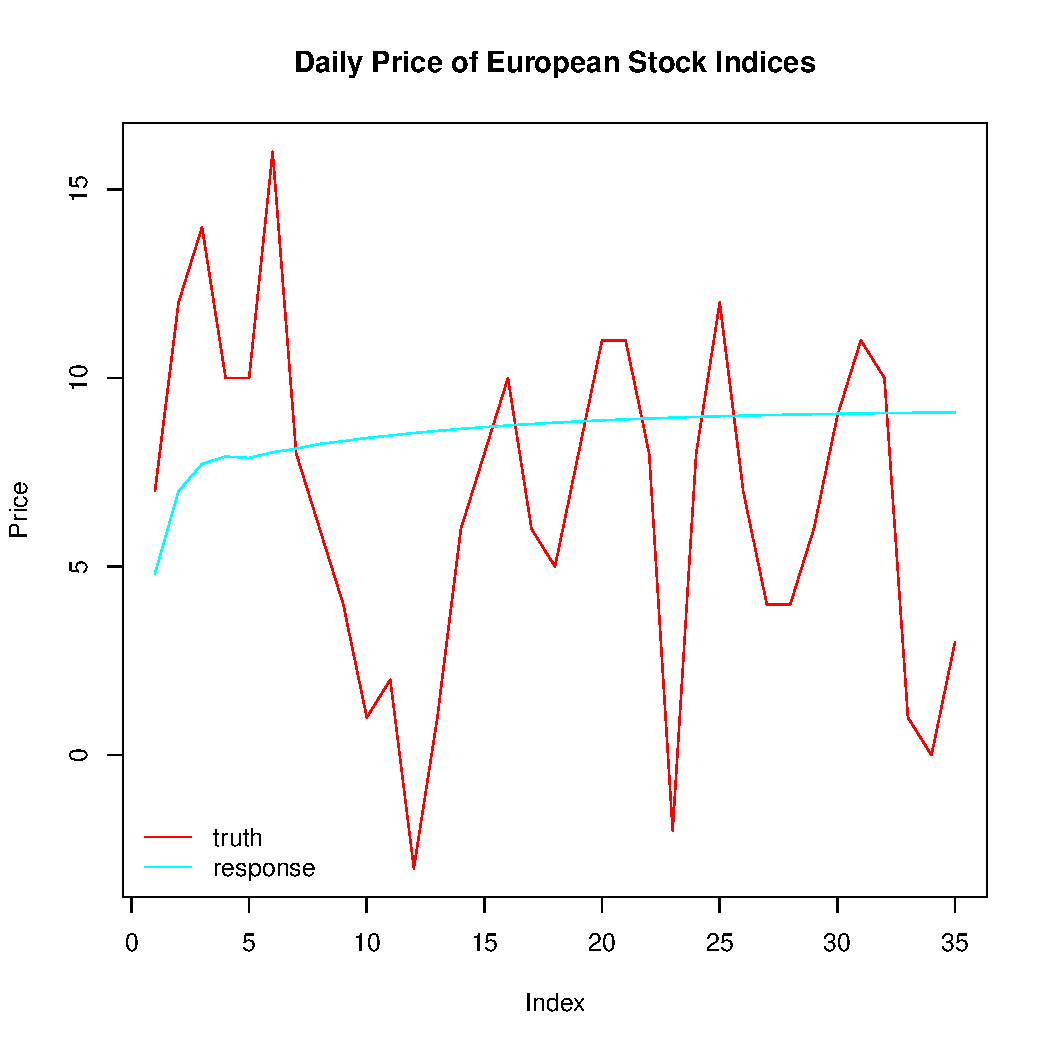
\includegraphics[width=\maxwidth]{figure/ensembleForecast5-1} 

\end{knitrout}
\doublespacing

\subsection{Multivariate Stacked Learner}
\label{sub:multiStack}

When there is a single target variable with multiple predictors stacked learning can be used with multivariate forecasters to forecast the predictors and have a machine learning model train over the forecasts of all variables. For this, equation~\ref{eq:ensemble} can be modified to include forecasts of other predictors $x_i,k$ where $k$ is the index for each predictor variable

\begin{equation}
\tilde{y}_{i+1} = \phi(\tilde{y}_{i+1,1},\dots, \tilde{y}_{i+1,m}, \tilde{x}_{i+1,1},\dots, \tilde{x}_{i+1,k}, \sum_{j=1}^m \epsilon_{i+1,j}, \sum_{j=1}^k \epsilon_{i+1,j})
\label{eq:ensembleMulti}
\end{equation}

In the example below, a boosted glm~\cite{glmboost} is used as a super learner over a sparse lag multivariate VAR model to forecast FTSE prices. A resampling strategy is creating for both the underlying stacked learner and the super learner.

\singlespacing
\begin{knitrout}
\definecolor{shadecolor}{rgb}{0.969, 0.969, 0.969}\color{fgcolor}\begin{kframe}
\begin{alltt}
\hlstd{multfore.task} \hlkwb{=} \hlkwd{makeMultiForecastRegrTask}\hlstd{(}\hlkwc{id} \hlstd{=} \hlstr{"bigvar"}\hlstd{,} \hlkwc{data} \hlstd{= eu.train,}
                                          \hlkwc{target} \hlstd{=} \hlstr{"FTSE"}\hlstd{)}

\hlstd{resamp.sub} \hlkwb{=} \hlkwd{makeResampleDesc}\hlstd{(}\hlstr{"GrowingCV"}\hlstd{,}
                              \hlkwc{horizon} \hlstd{=} \hlnum{32L}\hlstd{,}
                              \hlkwc{initial.window} \hlstd{=} \hlnum{.90}\hlstd{,}
                              \hlkwc{size} \hlstd{=} \hlkwd{nrow}\hlstd{(}\hlkwd{getTaskData}\hlstd{(multfore.task)),}
                              \hlkwc{skip} \hlstd{=} \hlnum{.01}
\hlstd{)}

\hlstd{resamp.super} \hlkwb{=} \hlkwd{makeResampleDesc}\hlstd{(}\hlstr{"CV"}\hlstd{,} \hlkwc{iters} \hlstd{=} \hlnum{3}\hlstd{)}
\end{alltt}
\end{kframe}
\end{knitrout}
\doublespacing

In \code{makeStackedLearner()}, the super learner argument contains the boosted glm model.

\singlespacing
\begin{knitrout}
\definecolor{shadecolor}{rgb}{0.969, 0.969, 0.969}\color{fgcolor}\begin{kframe}
\begin{alltt}
\hlstd{base} \hlkwb{=} \hlkwd{c}\hlstd{(}\hlstr{"mfcregr.BigVAR"}\hlstd{)}
\hlstd{lrns} \hlkwb{=} \hlkwd{lapply}\hlstd{(base, makeLearner)}
\hlstd{lrns} \hlkwb{=} \hlkwd{lapply}\hlstd{(lrns, setPredictType,} \hlstr{"response"}\hlstd{)}
\hlstd{lrns[[}\hlnum{1}\hlstd{]]}\hlopt{$}\hlstd{par.vals}\hlopt{$}\hlstd{verbose} \hlkwb{=} \hlnum{FALSE}


\hlstd{stack.forecast} \hlkwb{=} \hlkwd{makeStackedLearner}\hlstd{(}\hlkwc{base.learners} \hlstd{= lrns,}
                            \hlkwc{predict.type} \hlstd{=} \hlstr{"response"}\hlstd{,}
                            \hlkwc{super.learner} \hlstd{=} \hlkwd{makeLearner}\hlstd{(}\hlstr{"regr.glmboost"}\hlstd{,}
                                                        \hlkwc{family} \hlstd{=} \hlstr{"Laplace"}\hlstd{),}
                            \hlkwc{method} \hlstd{=} \hlstr{"growing.cv"}\hlstd{,}
                            \hlkwc{resampling} \hlstd{= resamp.sub)}
\end{alltt}
\end{kframe}
\end{knitrout}
\doublespacing

Just as with univariate stacked forecasting models, a parameter set is created for the multivariate VAR model and tuning is done with \code{tuneParams()}.

\singlespacing
\begin{knitrout}
\definecolor{shadecolor}{rgb}{0.969, 0.969, 0.969}\color{fgcolor}\begin{kframe}
\begin{alltt}
\hlstd{ps} \hlkwb{=} \hlkwd{makeParamSet}\hlstd{(}
  \hlkwd{makeDiscreteParam}\hlstd{(}\hlstr{"mfcregr.BigVAR.p"}\hlstd{,} \hlkwc{values} \hlstd{=} \hlnum{9}\hlstd{),}
  \hlkwd{makeDiscreteParam}\hlstd{(}\hlstr{"mfcregr.BigVAR.struct"}\hlstd{,} \hlkwc{values} \hlstd{=} \hlstr{"SparseLag"}\hlstd{),}
  \hlkwd{makeNumericVectorParam}\hlstd{(}\hlstr{"mfcregr.BigVAR.gran"}\hlstd{,} \hlkwc{len} \hlstd{=} \hlnum{2L}\hlstd{,} \hlkwc{lower} \hlstd{=} \hlnum{35}\hlstd{,}
                         \hlkwc{upper} \hlstd{=} \hlnum{50}\hlstd{),}
  \hlkwd{makeDiscreteParam}\hlstd{(}\hlstr{"mfcregr.BigVAR.h"}\hlstd{,} \hlkwc{values} \hlstd{=} \hlnum{32}\hlstd{),}
  \hlkwd{makeDiscreteParam}\hlstd{(}\hlstr{"mfcregr.BigVAR.n.ahead"}\hlstd{,} \hlkwc{values} \hlstd{=} \hlnum{32}\hlstd{)}
\hlstd{)}

\hlcom{## tuning}
\hlkwd{library}\hlstd{(parallelMap)}
\hlkwd{parallelStartSocket}\hlstd{(}\hlnum{4}\hlstd{)}
\hlkwd{configureMlr}\hlstd{(}\hlkwc{on.learner.error} \hlstd{=} \hlstr{"warn"}\hlstd{)}
\hlkwd{set.seed}\hlstd{(}\hlnum{1234}\hlstd{)}
\hlstd{multfore.tune} \hlkwb{=} \hlkwd{tuneParams}\hlstd{(stack.forecast, multfore.task,}
                           \hlkwc{resampling} \hlstd{= resamp.sub,}
                           \hlkwc{par.set} \hlstd{= ps,} \hlkwc{control} \hlstd{=} \hlkwd{makeTuneControlGrid}\hlstd{(),}
                           \hlkwc{measures} \hlstd{= mase,} \hlkwc{show.info} \hlstd{=} \hlnum{FALSE}\hlstd{)}
\hlkwd{parallelStop}\hlstd{()}
\hlstd{multfore.tune}
\end{alltt}
\end{kframe}
\end{knitrout}

\begin{knitrout}
\definecolor{shadecolor}{rgb}{0.969, 0.969, 0.969}\color{fgcolor}\begin{kframe}
\begin{verbatim}
## Tune result:
## Op. pars: mfcregr.BigVAR.p=5; mfcregr.BigVAR.struct=SparseLag; mfcregr.BigVAR.gran=30,30; mfcregr.BigVAR.h=32; mfcregr.BigVAR.n.ahead=32
## multivar.mase.test.mean=0.453
\end{verbatim}
\end{kframe}
\end{knitrout}
\doublespacing

Once the tuning is complete, the best model can be extracted with \code{setHyperPar2()} and the final model will be trained on all of the data. Since we are using the multivariate model to produce forecasts for an singel variable, univariate MASE is use instead of the multivariate form of MASE.

\singlespacing
\begin{knitrout}
\definecolor{shadecolor}{rgb}{0.969, 0.969, 0.969}\color{fgcolor}\begin{kframe}
\begin{alltt}
\hlstd{stack.forecast.f}  \hlkwb{=} \hlkwd{setHyperPars2}\hlstd{(stack.forecast,multfore.tune}\hlopt{$}\hlstd{x)}
\hlstd{multfore.train} \hlkwb{=} \hlkwd{train}\hlstd{(stack.forecast.f,multfore.task)}
\end{alltt}
\end{kframe}
\end{knitrout}



\begin{knitrout}
\definecolor{shadecolor}{rgb}{0.969, 0.969, 0.969}\color{fgcolor}\begin{kframe}
\begin{alltt}
\hlstd{multfore.pred} \hlkwb{=} \hlkwd{predict}\hlstd{(multfore.train,} \hlkwc{newdata} \hlstd{=} \hlkwd{as.data.frame}\hlstd{(eu.test))}
\hlstd{multfore.pred}
\end{alltt}
\begin{verbatim}
## Prediction: 32 observations
## predict.type: response
## threshold: 
## time: 0.02
##                      truth response
## 1998-07-12 07:50:46 5960.2 5629.466
## 1998-07-13 17:32:18 5988.4 5629.378
## 1998-07-15 03:13:50 5990.3 5629.423
## 1998-07-16 12:55:23 6003.4 5629.519
## 1998-07-17 22:36:55 6009.6 5629.655
## 1998-07-19 08:18:27 5969.7 5629.759
## ... (32 rows, 2 cols)
\end{verbatim}
\begin{alltt}
\hlkwd{performance}\hlstd{(multfore.pred, mase,} \hlkwc{task} \hlstd{= multfore.task)}
\end{alltt}
\begin{verbatim}
##      mase 
## 0.2363337
\end{verbatim}
\end{kframe}
\end{knitrout}
\doublespacing
\begin{knitrout}
\definecolor{shadecolor}{rgb}{0.969, 0.969, 0.969}\color{fgcolor}
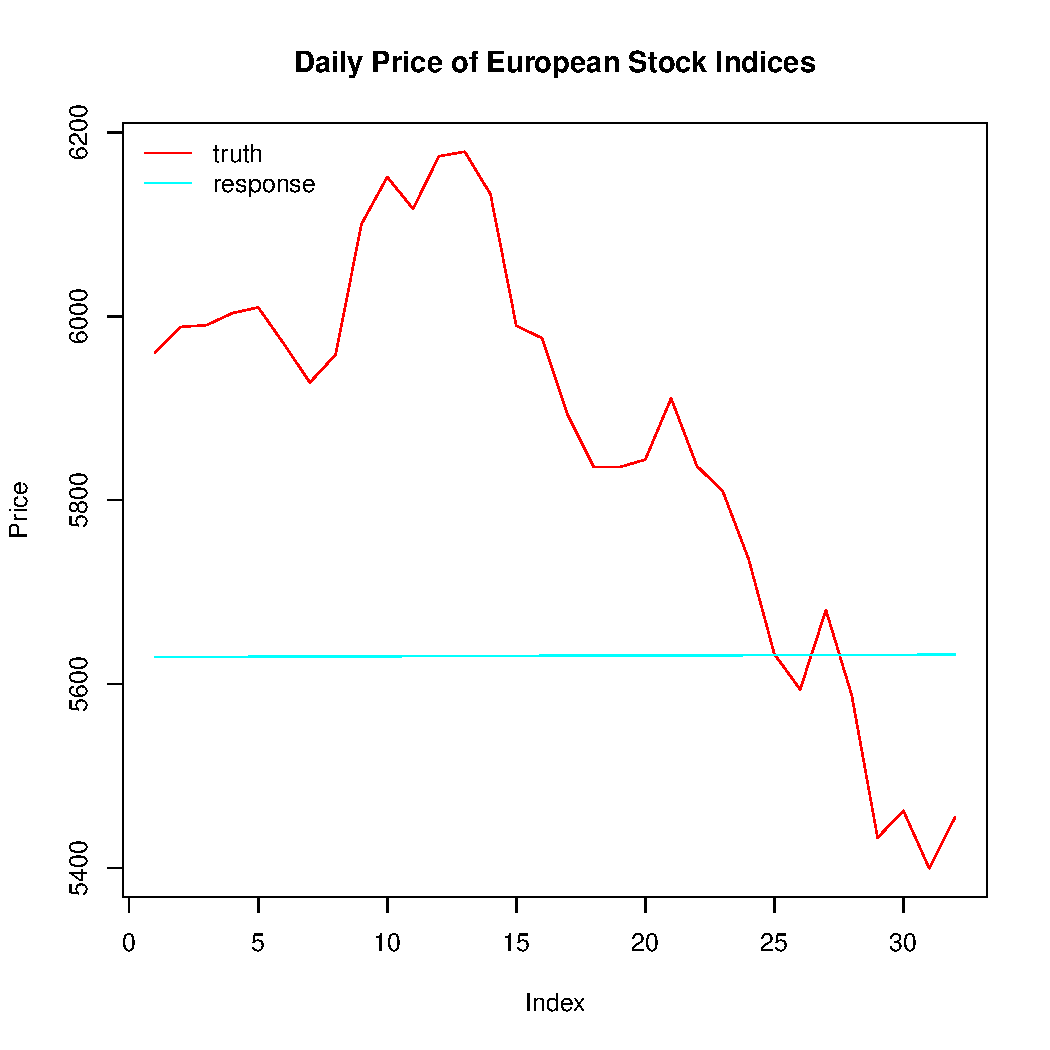
\includegraphics[width=\maxwidth]{figure/multiForecast8-1} 

\end{knitrout}

\section{Conclusion}

The results of this paper show that creating a unified interface for forecasting models in \proglang{R} allows for better models through an automated methedology of resampling, preprocessing, model selection, stacking tuning, and training. Building on the wide range of forecasting packages available in \proglang{R}, automating tasks such as windowing cross validation and model selection allow applied forecasters to spend less time dealing with the beauracracy of modeling and more time testing new models. New methods such as multivariate stacked learners, Lambert W transforms, and the ability to create arbitary AR($p,d$) machine learning models allows researchers to easily experiment with new ideas. While the example models here are not perfect, this was mostly due to time. It will be easy for researchers to beat the models created in this paper.

Multivariate stacked learners are quite new, and to this researchers knowledge have not been used in this context. Future research based on this package would involve tuning these models to see how useful they are in the real world. Classification forecast made available in this extension is a very new field, and with the ease of making these models new research in this area can progress much quicker. Updates to this package will include more multivariate and univariate forecast learners as well as new methods to stack models such as Bayesian averaging~\cite{bayesianAverage}.

%\small
\bibliography{thesisbib}{}
\bibliographystyle{plain}

\end{document}
